% Domenico Giusti

% Paläoanthropologie,
% Senckenberg Centre for Human Evolution and Palaeoenvironment (HEP) &
% Eberhard Karls Universität Tübingen

% Institut für Naturwissenschaftliche Archäologie (INA),
% Eberhard Karls Universität Tübingen
% Rümelinstr. 23, 72070 Tübingen, Raum 509

% Off.: +49 7071 2974077
% Mob.: +49 (0)176 68100672
% Mob.: +30 6946293471
% Mob.: +39 3936476718

% domenico.giusti@uni-tuebingen.de
% domenico.giusti@senckenberg.de

% LaTeX manuscript -- English {elsarticle}

\documentclass[review,times,authoryear]{elsarticle} %%[preprint/review/5p]

\usepackage[T1]{fontenc}
\usepackage[utf8]{inputenc}
\usepackage[english]{babel}

\usepackage{natbib}
\biboptions{sort}
\usepackage[colorlinks]{hyperref}
\usepackage{lineno}
\usepackage{textcomp}
\usepackage{amsmath}
\usepackage{rotating}

%% add for two columns (5p) preprint
%\usepackage{dblfloatfix}

\journal{Boreas} %% Boreas: British (UK) English

\begin{document}

\begin{frontmatter}
  
  \title{Recursive anisotropy: A spatial taphonomic study of the Early Pleistocene vertebrate assemblage of Tsiotra~Vryssi, Mygdonia Basin, Greece}
  
  \author[tue]{D.~Giusti\corref{cor1}}
  \ead{domenico.giusti@uni-tuebingen.de}
  \cortext[cor1]{Corresponding author}
  
  \author[tue]{G.~E.~Konidaris}
  \author[tue]{V.~Tourloukis}
  \author[mi]{M.~Marini}
  \author[mi]{M.~Maron}
  \author[mi]{A.~Zerboni}
  \author[tue]{N.~Thompson}
  \author[thess]{G.~D.~Koufos}
  \author[thess]{D.~S.~Kostopoulos}
  \author[tue]{K.~Harvati}
  
  \address[tue]{Paläoanthropologie, Senckenberg Centre for Human Evolution and Palaeoenvironment, Eberhard Karls Universität Tübingen, Rümelinstr. 23, 72070 Tübingen, Germany}
  \address[mi]{Università degli Studi di Milano, via Mangiagalli 34, 20133 Milano, Italy}
  \address[thess]{Aristotle University of Thessaloniki, Department of Geology, Laboratory of Geology and Palaeontology, 54124 Thessaloniki, Greece}

  \begin{abstract} %% maximum 200 words
    By applying advanced spatial statistical methods, spatial taphonomy complements the traditional taphonomic approach and enhances our understanding of biostratinomic and diagenetic processes. In this study, we elaborate on a specific aspect - spatial anisotropy - of taphonomic processes. We aim to unravel the taphonomic history of the Early Pleistocene vertebrate assemblage of Tsiotra Vryssi (Mygdonia Basin, Macedonia, Greece). Circular statistics are used for the fabric analysis of elongated elements; geostatistics (directional variograms), wavelet and point pattern analyses are applied for detecting anisotropy at the assemblage level. The anisotropy of magnetic susceptibility (AMS) of sedimentary magnetic minerals is as well investigated. The results of our analyses, integrated with preliminary remarks about the differential preservation of skeletal elements, sedimentological and micromorphological observations, suggest multiple dispersion events and recurrent spatial re-arrangement of a lag, (peri)autochthonous assemblage, consistent with the cyclical lateral switching of a braided fluvial system. Furthermore, this study offers an important contribution to the building of a spatial taphonomic referential framework for the interpretation of other fossil vertebrate assemblages, including archaeo-palaeontological ones.
  \end{abstract}
  
  \begin{keyword} %% maximum of 6 keywords
    Anisotropy \sep Spatial taphonomy \sep Taphonomy \sep Site formation processes \sep Early Pleistocene \sep Greece
  \end{keyword}
  
\end{frontmatter}

\linenumbers

\section{Introduction}

%% Theoretical framework: taphonomy & spatial taphonomy
Since the first definition of taphonomy as ``the study of the transition (in all its details) of animal remains from the biosphere into the lithosphere'' \citep{Efremov1940}, the spatial properties of taphonomic processes received special attention. Concerned about thanatocoenosis, \cite{Efremov1940} indicated as chief part of a taphonomic study, among others, the analysis of ``the spatial distribution of animal remains and their distribution relatively to the planes of stratification''. More recent research on early hominid evolution \citep{Behrensmeyer1975,Boaz1976,Hill1976} extended the original definition of taphonomy beyond its role as a ``new branch of paleontology'' \citep{Efremov1940} to include also formation and modification processes of the archaeological record. Despite some misrepresentations in the archaeological adaptation of the original concept (e.g., the ontological difference between natural and cultural formation processes; \citealp{Lyman2010,Dominguez-Rodrigo2011}), in the last decades taphonomy has widened its theoretical and methodological framework towards an integrative and multidisciplinary investigation that aims to reconstruct the past in all its details, incorporating any signal of the processes, both natural and cultural, that modified the original properties of the organic and inorganic components \citep{Dominguez-Rodrigo2011}.

If taphonomy evolved towards an evolutionary and systemic approach that embraces multiple taphonomic levels of organisation (i.e., basic taphonomic elements, taphonomic groups [taphons], taphonomic populations and taphoclades; \citealp{Fernandez-Lopez2006}), likewise, the study of the spatial properties of taphonomic processes extended from the analysis of the spatial distribution of animal remains in relation to the stratigraphic setting, towards a multilevel quantitative investigation of the spatial behaviour of different taphonomic entities \citep[\emph{sensu}][]{Fernandez-Lopez2006}. Therefore, spatial taphonomy \citep{Giusti2016,Dominguez-Rodrigo2017}, encompasses the spatial properties of basic entities (i.e., taphonomic elements, constituting the fossil record), as well as higher level entities (e.g., taphonomic groups or populations). Indeed, at multiple scales and levels of organisation, the spatial patterns observed in any palaeontological or archaeological assemblage retain valuable information about taphonomic accumulation and re-elaboration processes \citep[\emph{sensu}][]{Fernandez-Lopez2002}. Spatial taphonomic data, appropriately recorded, can be quantitatively analysed within a statistical framework in order to reliably draw inferences about taphonomic processes, in turn with consequences for palaeoecological reconstructions \citep{Fernandez-Jalvo2011}, biochronological estimates and the interpretation of past human behaviours.

%% Recurrent anisotropy & fluvial processes
In this study, we elaborate on a specific aspect - anisotropy - of the spatial properties of taphonomic entities, with implications for the interpretation of taphonomic processes. Anisotropy, as opposed to isotropy, is generally defined as the property of a process of being directionally dependent. Spatial anisotropic patterns can be seen as products of physical anisotropic processes, such as fluvial or eolian processes, which modified at multiple scales and levels of organisation the original spatial properties of taphonomic entities.

At the level of basic taphonomic elements, anisotropy, expressed as preferential orientation of fossils or artefacts, is among the key variables used for interpreting site formation and modification processes. Especially in terrestrial alluvial environments, anisotropy is one of the proxies traditionally used to discriminate autochthonous vs. allochthonous assemblages \citep[][among others]{Petraglia1987,Petraglia1994,Schick1987a,Toots1965,Voorhies1969}. The orientation of elongated elements, prone to preferentially align along the flow direction, would eventually indicate the action of water-flows and suggest substantial transport prior to burial. Nevertheless, anisotropy has been equally documented in autochthonous assemblages subjected to low-energy water-flows \citep{Cobo-Sanchez2014,Dominguez-Rodrigo2012,Dominguez-Rodrigo2014}; hence, it can be a necessary but not sufficient condition to differentiate allochthony from autochthony \citep{Lenoble2004}. Moreover, besides water-flow processes, anisotropy has been as well observed in association with a wide range of other biostratinomic processes, such as slope processes \citep{Bertran1995} and trampling \citep{Benito-Calvo2011a}.

Although the anisotropy of basic taphonomic elements have been long studied, the anisotropy of higher level taphonomic entities received by far less attention (see \citealp{Markofsky2012} for a directional analysis of archaeological surface distributions). Here we address this research gap and conduct a spatial taphonomic study of anisotropy both at the level of fossil specimens and at the assemblage level. The present study uses a comprehensive set of spatial statistics (fabric analysis, geostatistics, wavelet analysis, point pattern analysis) in order to identify directional trends that may not be readily apparent. Indeed, beyond the traditional approach of eye-spotting spatial patterns, spatial statistics allow one to adopt a more formal, quantitative approach.

Furthermore, at the scale of sedimentary particles, anisotropy is investigated by means of anisotropy of magnetic susceptibility (AMS). AMS refers to the property of elongated magnetic crystals to orient parallel to the flow direction when transported as sedimentary clasts. In sedimentology, AMS analysis is widely applied in order to determine paleoflows in a range of depositional environments, including turbidite systems, contouritic drifts, beaches, deltas and tidal flats \citep[][among others]{Lowrie1987,Liu2001,Pares2007,Novak2014,Felletti2016}.

%% Main aims
Therefore, integrating the results of our multiscale and multilevel analysis of anisotropy with preliminary remarks about differential taphonomic preservation, sedimentological and micromorphological observations, we aim to disentangle the taphonomic history of the fossiliferous locality Tsiotra~Vryssi (Mygdonia Basin, Macedonia, Greece; \citealp{Konidaris2015}).

Finally, this study offers an important contribution to the building of a spatial taphonomic referential framework for the interpretation of other fossil vertebrate assemblages, including archaeo-palaeontological ones \citep{Dominguez-Rodrigo2017}.

\section{The palaeontological site of Tsiotra Vryssi (TSR)}

%% Geographical and geological setting (Mygdonia Basin)
Tsiotra~Vryssi (TSR) is located in the Mygdonia Basin (Macedonia, Greece), about 45~km Southeast of Thessaloniki (Fig.~\ref{fig:1}). TSR was discovered in 2014 by a joint research team from the Aristotle University of Thessaloniki and the Eberhard Karls University of Tübingen during systematic field surveys in the basin. After the first collection of fossils from the exposed natural section and the test excavation carried out in 2014, systematic excavation of the site took place in 2015 and is still ongoing (Fig.~\ref{fig:pics}a).

To date, the excavation covers about a 10 m-thick stratigraphic interval from the upper Gerakarou Formation (Fig.~\ref{fig:1}), a suite of continental clastic deposits of mainly fluvial origin and inter-layered paleosols \citep{Koufos1995,Konidaris2015}. The TSR fauna occurs mainly within a c. 1 m-thick interval of silts (uppermost part of unit Geo2, see Fig~\ref{fig:log}) and comprises several mammalian taxa, as well as some birds and reptiles, whose preliminary biochronological correlation is consistent with a late Villafranchian (Early Pleistocene) age \citep{Konidaris2015,Konidaris2016}.

\begin{figure*}[]
  \centering
  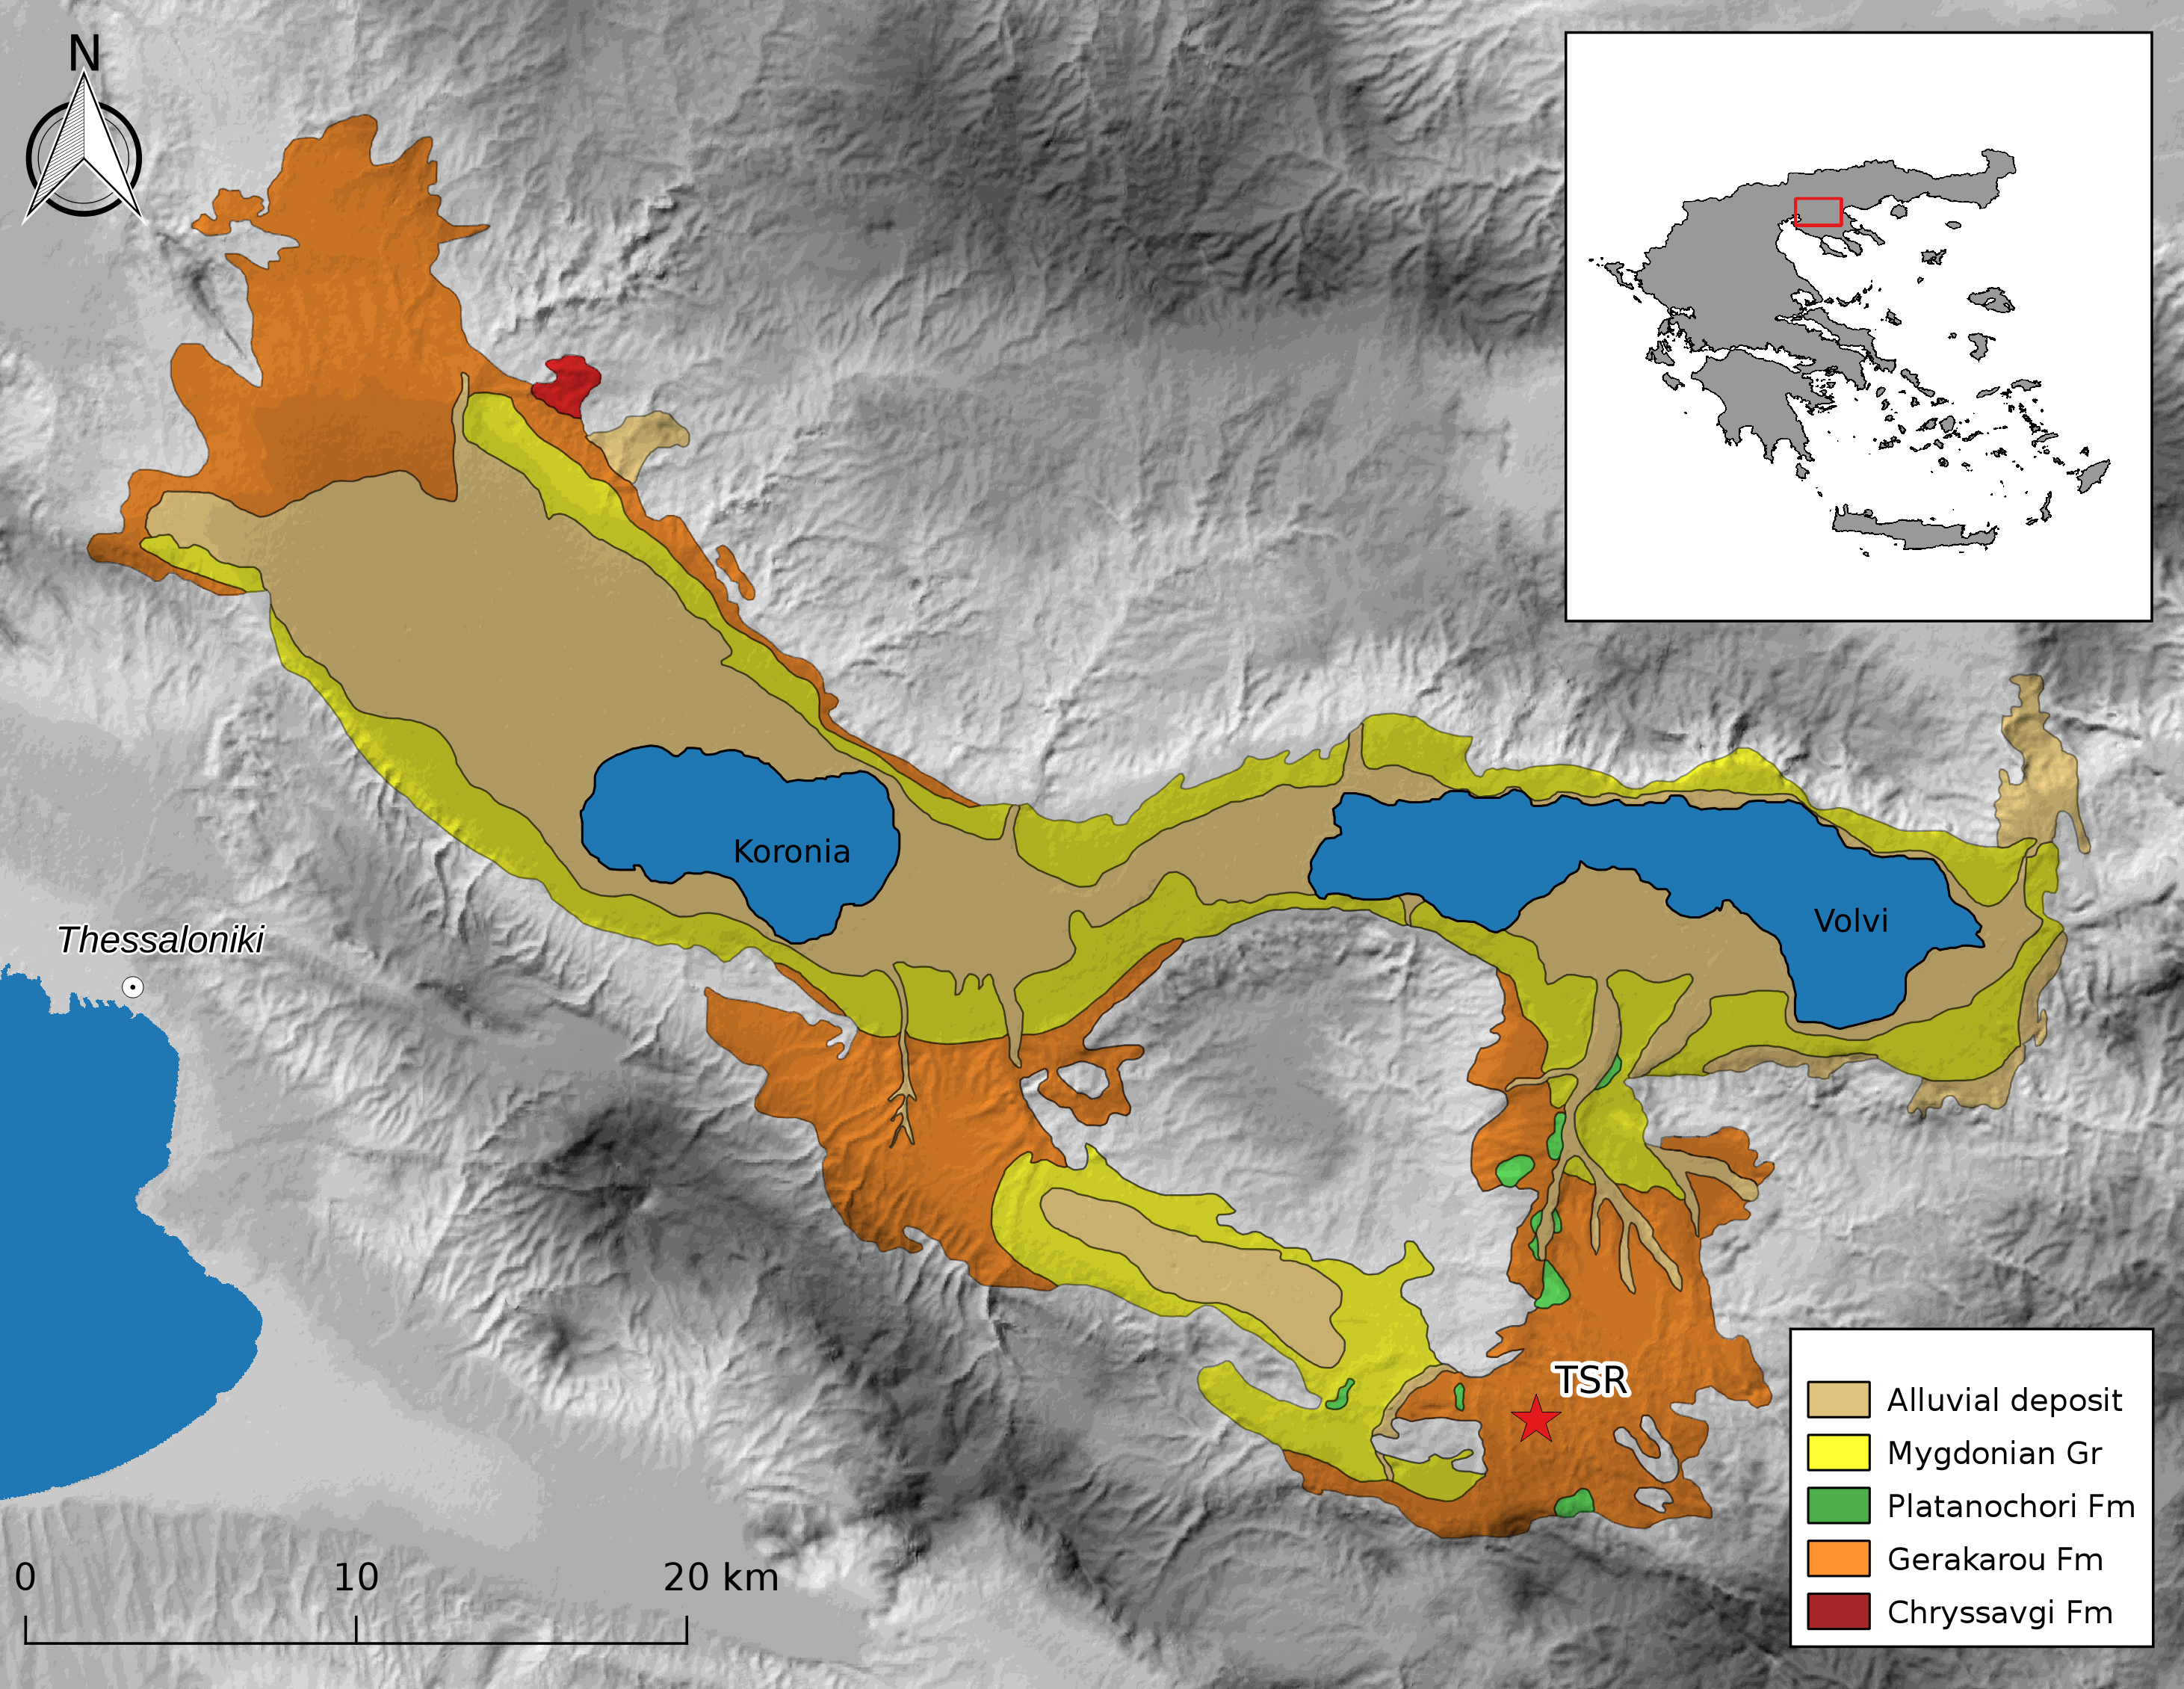
\includegraphics[width=1\textwidth]{artwork/Fig1.png}
  \caption{Geological setting of the Mygdonia Basin (Macedonia, Greece) showing the Neogene and Quaternary lithostratigraphic units and the location of Tsiotra~Vryssi (TSR), modified after \cite{Koufos1995}}
  \label{fig:1}
\end{figure*}

\begin{figure*}[]
  \centering
  \includegraphics[width=.85\textwidth]{artwork/Fig2.png}
  \caption{Panoramic view (2017) of the excavation area of Tsiotra Vryssi. Pictures of articulated specimens (a, b, c, d) and clusters of bones (e, f).}
  \label{fig:pics}
\end{figure*}

%% Stratigraphic setting
Two main depositional units are identified (Geo 1 and Geo 2, from younger to older; Fig.~\ref{fig:log}). The fossiliferous unit Geo 2 begins with $\sim$1.5 m (Geo 2b in Fig.~\ref{fig:log}) of cross-stratified gravelly sands organised into dm-thick beds with a range of planar to trough-cross laminations. Noteworthy, Geo 2b can be followed laterally for at least 150m in the E-W direction, suggesting an extensive setting of deposition. Above a sharp contact, a few tens of cm of well-sorted, structure-less fine sands follow, which rapidly grade upward into the deposit forming the matrix of the main TSR fossil assemblage (Geo 2a in Fig.~\ref{fig:log}). This is represented by $\sim$1 m of poorly sorted silts (moderately rich in mica grains), locally intercalated by cm-thick lenses of medium-coarse grained sands and relatively more clayey in the uppermost 30 cm of the deposit. Apart for alignment of isolated sand to granule grade clasts and some crude parallel lamination in coarse lenses, the deposits appear overall structure-less. Typically, Geo 2a has a very pale brown colour with a few (less than 10\%) pink to reddish yellow mottles, whereas the topmost part of Geo 2a has a strong brown to dark yellowish brown matrix with about the 15-20\% of reddish yellow mottles. This change in colour is associated with the occurrence of very small calcareous nodules and common to abundant Mn-Fe-bearing nodules with diameter less then 1 cm (see micromorphological analysis in Section~4.5).

Geo 1b is represented by an up to 2 m-thick bed set of cross-stratified gravelly sands and gravels, similar to those observed in Geo 2b (Fig.~\ref{fig:log}). It sits on top of a basal erosion, down-cutting deeply into older sediments (Geo 2a) and shallowing toward the West. In the same direction, the Geo 1b beds tend to be thinner, finer grained and less extensive laterally, suggesting less energetic hydrodynamic conditions. Though poorly exposed, the younger Geo 1a is represented by a monotonous 3 m-thick section of poorly silty sands devoid of coarse intercalations, which rapidly grades into clayey silts of a distinctive pale brown colour.

\begin{sidewaysfigure}[]
%\begin{figure*}[]
  \centering
  \includegraphics[width=1\textwidth]{artwork/Fig3.png}
  \caption{Stratigraphic sedimentary logs (log1 and log 2) with location of main erosional surfaces bounding depositional units Geo 1 and Geo 2, block samples TVB-Z 1 and 2 collected for micromorphology analysis and interval sampled for anisotropy of magnetic susceptibility analysis (AMS); b) WNW-ESE oriented panoramic view of the excavation site and location of the stratigraphic log2 in the background; c) and d) are details of the lower half of log2 showing the basal erosion of Geo 1b followed upward by inclined laminations; e) the middle part of Geo 2a (i.e., the fossiliferous unit) sampled for AMS analysis. Note the presence of cm-thick sand lenses of sands with Fe-hydroxide stains; f) detail of cross stratifications from the top of Geo 2b.}
  \label{fig:log}
%\end{figure*}
\end{sidewaysfigure}

%% Spatial distribution
Overall, the stratigraphic position of TSR in the fluvioterrestrial Gerakarou Formation \citep{Koufos1995} and the specific sedimentary sequence of the site indicate that the TSR assemblage formed in a relatively low energy fluvial environment. A preliminary visual inspection of the vertical and horizontal distribution of the fossil finds (Fig.~\ref{fig:map}) suggests a densely preserved association of fossils (about 24 elements/m$^2$), homogeneously distributed within the study area. Apparent anisotropy is also suggested at assemblage level.

\begin{figure*}[]
  \centering
  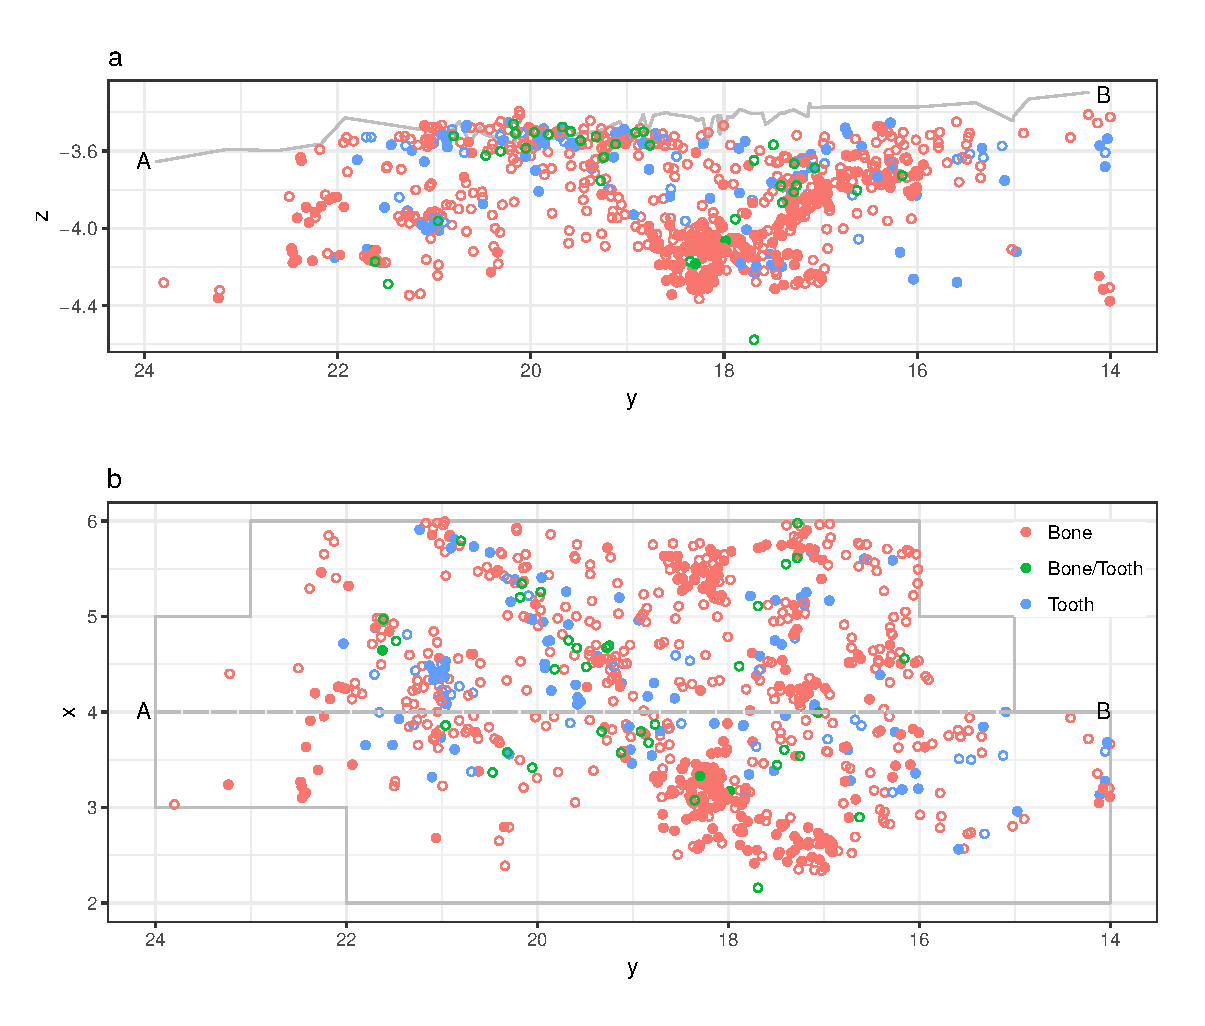
\includegraphics[width=1\textwidth]{artwork/Fig4.pdf}
  \caption{Vertical (a) and horizontal (b) distribution of the sampled fossil specimens from Tsiotra Vryssi (excavations 2015-2017). Filled circles mark complete specimens, hollow circles mark fragmented ones. Grey continuous line in a) marks the Geo 1/2 erosional contact, as recorded at the AB transect marked in b).}
  \label{fig:map}
\end{figure*}

%% Main aims
In such a fluvial depositional context, questions arise with respect to the specific character of the TSR fossil assemblage, the number of depositional events (single or multiple) and the degree of transportation of the fossil record (autochthonous vs. allochthonous assemblage).

\section{Material and methods}

\subsection{Data collection and sub-setting}

%% Excavation protocol
Since 2015 a grid of 1 m$^2$ units was set up and a total station was used in order to record the spatial provenience of collected (i.e., diagnostic bones and teeth, and carnivore modified bones) and not collected remains (i.e., non-diagnostic bone fragments with length $\geq$50~mm; Fig.~\ref{fig:pics}a). Non-diagnostic, or non-carnivore modified bone fragments with length $<$50~mm were not recorded. This dimensional threshold was chosen because small bone fragments show more random orientations than longer specimens \citep{Dominguez-Rodrigo2014}. Orientation (plunge and bearing) of clearly elongated specimens (i.e., specimens with length at least twice the width) was measured with a 1~degree accuracy, using a compass and inclinometer \citep[][among others]{Voorhies1969,Fiorillo1991,Eberth2007}. Strike and dip measurements were taken along the symmetrical longitudinal a-axis (SLA) of the specimens \citep{Dominguez-Rodrigo2013}, using the lowest endpoint of the a-axis as an indicator of the vector direction. The dimensions (length and maximum width) of the recorded finds were measured on-site with a millimetric measuring tape.

%% Sample (Mammalia:738, NA:75, Aves:15, Reptilia:7, ?Reptilia:2, ?:4)
The present spatial taphonomic study analysed a sample of stratified specimens (n = 797) from the fossiliferous unit Geo 2a, whose spatial coordinates were recorded with the total station. The area of analysis comprises the 34 m$^2$ excavated from 2015 until 2017. The sample included mostly macromammal remains (n = 707, 89\%), undetermined isolated bone fragments (n = 70), birds (n = 12) and turtle (n = 8) remains. A sub-sample (n = 249) was further subset for the fabric analysis described below. Stratified specimens from Geo 2a collected during the test excavation of 2014, or subsequently found in plaster-jackets with concentration of bones during the lab preparation were excluded due to the lack of precise spatial coordinates. The very small sample (n = 4) of micromammal remains was also not included in the spatial and faunal analyses. Faunal analysis was conducted on a sub-sample of complete or fragmented, isolated or articulated macromammal remains (n = 707). Further sub-setting strategies are described below.

%% Micromorph/AMS
As for the AMS analysis, we collected 18 cylindrical oriented samples (Ø = 2.5 cm) from the middle part of the fossiliferous unit Geo 2a (Fig.~\ref{fig:log}). AMS analysis was performed at the Alpine Laboratory of Paleomagnetism in Peveragno (Italy) using a AGICO KLY-3 Kappabridge susceptibility meter (15-positions, manual oriented).

In order to investigate the micromorphological properties of the Geo 2a unit (i.e., sedimentary structures and pedogenetic features), two blocks of undisturbed sediment were collected from the excavation area; one (TVB-Z 1) from the middle part of the unit and the other (TVB-Z 2) from the topmost 30 cm of it (Fig.~\ref{fig:log}). The blocks were later consolidated for preparation of thin sections following the methods described in \citet{Murphy1986}).

\subsection{Spatial anisotropy}

%% Intro
Different methods have been developed in neighbouring disciplines to detect spatial anisotropy. Here we use circular statistics for the fabric analysis of taphonomic elements; geostatistics (directional variograms), wavelet analysis and point pattern analysis for detecting anisotropy at the assemblage level.

\subsubsection{Fabric analysis}

%% Intro
The first controlled experiments and analyses of the orientation and dispersal of disarticulated  mammal bones as indicators of the depositional context, carried out by \cite{Toots1965} and \cite{Voorhies1969}, led to an increasing number of studies on the effects of water flows on natural and anthropogenic faunal assemblages \citep[][among others]{Nash1987,Schick1987a,Petraglia1987,Petraglia1994,Fiorillo1991,Benito-Calvo2011,Torre2013a,Dominguez-Rodrigo2012,Dominguez-Rodrigo2014,Dominguez-Rodrigo2014c,Cobo-Sanchez2014,Aramendi2017,Organista2017}.

Whereas most of these studies have been conducted on disarticulated long bones or elongated bone fragments - which were observed to preferentially align their a-axes along the direction of the flow - relatively few have investigated the hydraulic behaviour of articulated skeletal elements. Flume experiments conducted by \cite{Coard1995} and \cite{Coard1999} demonstrated that articulated bones display a greater transport potential than disarticulated ones when the articulated elements align themselves. However, they also noted that skeletal parts with a higher number of articulated elements, such as complete limbs, may show weak preferential orientation when assuming disorganised spatial configuration, i.e., when not aligned. Therefore, articulated bones, although relatively common at TSR (Fig.~\ref{fig:pics}a,b,c,d), were not included in the fabric analysis.

%% Subset & Methods
In this study we applied circular statistics to a subset of 249 non-articulated, elongated bone specimens, having length >= 20mm \citep{Dominguez-Rodrigo2014}. No distinction of skeletal elements was made, due to the high percentage (91\%, n = 227) of fragmented remains in the analysed sample - mostly appendicular (n = 122), undetermined (n = 93), axial and cranial (n = 12) fragments - and due to the low percentage (9\%, n = 22) of complete bones - 17 limb bones, 4 scapulae and a rib.

We applied Rayleigh and omnibus tests of uniformity, such as Kuiper, Watson and Rao \citep{Jammalamadaka2001}, to test the isotropic orientation of the fossil specimens. Whereas the Rayleigh test assumes a unimodal distribution and assess the significance of the sample mean resultant length ($\bar{R}$), the omnibus tests detect multimodal departures from the null hypothesis of circular isotropy.

Rose and equal area Schmidt diagrams were used as exploratory data analysis tools to visualise the sample distribution. Compared to the widely used rose diagrams, which plot the circular distribution of the bearing values, the Schmidt equal area diagram informs about the distribution of the three-dimensional orientation (plunge and bearing) of the elements \citep{Fiorillo1988}. Points plotting at the margin of the globe indicate planar fabric, whereas points towards the centre have higher dip angles.

The Woodcock diagram \citep{Woodcock1983}, based on three ordered normalised eigenvalues ($S_1$, $S_2$, $S_3$), was used to discriminate between linear (cluster), planar (girdle) and isotropic distributions. In the Woodcock diagram, the $C$ parameter ($C=ln(S_1/S_3)$) expresses the strength of the preferential orientation, and its significance is evaluated against critical values from simulated random samples of different sizes. A perfect isotropic distribution would plot at the origin, with equal eigenvalues ($S_1=S_2=S_3=1/3$). On the other hand, the $K$ parameter ($K=\frac{ln(S_1/S_2)}{ln(S_2/S_3)}$) expresses the shape of the distribution, and it ranges from zero (uni-axial girdles) to infinite (uni-axial clusters).

%% Assumptions & Expectations
In a fluvio-lacustrine environment a cluster distribution would suggest a strong preferential orientation of the sample, such as in the case of channelised water flows \citep{Petraglia1994}, whereas a girdle distribution a weaker preferential orientation, spread over a wider range of directions. Overland flows have been interpreted to produce such a pattern \citep{Organista2017}. On the other hand, a isotropic distribution would suggest that post-depositional disturbance by water flows was not strong enough to preferentially orient the assemblage \citep{Dominguez-Rodrigo2014c}. However, a variety of taphonomic processes can produce similar patterns. Fabric analysis, although very informative, has low power by itself. In order to overcome the intrinsic limitations of the fabric analysis, a multivariate approach to site formation and modification processes should be employed \citep{Lenoble2004}.

\subsubsection{Geostatistics}

%% Intro
Geostatistics refer to a body of concepts and methods typically applied to a limited sample of observations of a continuous variable, for example environmental variables. Geostatistics thus aim to estimate the variance and spatial correlation of known observations and predict, using interpolation methods such as Kriging, unknown values of the variable at non-observed locations. Moreover, by using directional variograms, geostatistics enable the identification of spatial anisotropy (i.e., directional patterns). Since the vast majority of spatial statistics assume stationarity and isotropy, it is well understood that a misinterpretation of spatial anisotropy may result in inaccurate spatial modelling and prediction.

Although well known in ecological studies, only a relatively small number of studies have explicitly applied geostatistics to the study of site formation and modification processes, using directional variograms to investigate the specimens size spatial distributions \citep{Dominguez-Rodrigo2014b,Dominguez-Rodrigo2014c}, or to specifically detect spatial anisotropy of archaeological assemblages \citep{Bevan2009,Markofsky2012}.

%% Subset & Methods
In order to investigate spatial anisotropy in the distribution of the TSR fossil assemblage and identify spatial continuity in some directions more than others, we used directional variograms and variogram maps. The studied sample includes 797 recorded specimens (isolated or articulated, complete or fragmented bones and teeth) unearthed from Geo 2a and included in the 34 m$^2$ window of analysis (Fig.~\ref{fig:map}). The same sample was used for the wavelet and point pattern analyses.

Specifically, plotting the semi-variance between the variable values of sampled point pairs as a function of distance (spatial lag) between these pairs, directional variograms are used to model the spatial variation at multiple scales and different directions. Three parameters (\emph{nugget}, \emph{range} and \emph{sill}) are estimated from an experimental variogram to fit a theoretical omnidirectional variogram. The \emph{nugget} is used to account for spatial variability at very short distances. The \emph{range} indicates the maximal distance up to which there is spatial correlation. At longer distances the semi-variance levels off forming the \emph{sill}, indicating independence between pairs of sample separated by that minimum distance \citep{Dale2014,Lloyd2004}. Thus, we plotted the experimental directional variogram against the theoretical omnidirectional variogram. A directional semi-variance lower than the fitted omnidirectional variogram indicates continuity in the analysed direction. We selected for our analysis the N-S (0°), E-W (90°), NE-SW (45°) and NW-SE (135°) geographical directions. In addition to the directional variograms, variogram maps are visual representations of the semi-variance: the anisotropy is represented by an ellipse, its axes being proportional to the variation expected in each direction. Thus, the direction of maximum anisotropy corresponds with the major axis of the ellipse \citep{Legendre2012}.

\subsubsection{Wavelet analysis}

%% Intro
As a second method for the detection of spatial anisotropy at the assemblage level we used the wavelet analysis. Wavelet analysis, commonly applied in mathematics for signal processing, has relatively wide application in palaeoclimatology and palaeoecology, but is seldom used in studies on site formation processes \citep{Markofsky2012}.

%% Subset & Methods
Unlike the geostatistics approach to the analysis of spatial anisotropy, which is based on a transformation of point values into a continuous surface, the wavelet approach does not apply any transformation, but identifies the elements (points) of a pattern merely by their location. In this regard, the wavelet analysis does not suffer from the arbitrary choice of a surface smooth parameter, as in the case of geostatistics.

For each specific point of the pattern, a wheel of 360 sectors of 1° is used to measure the average variance in the angles between point pairs \citep{Rosenberg2004}. The significance of the wavelet analysis is evaluated against 199 Monte Carlo simulations of the observed pattern under the null hypothesis of randomness. The variance is plotted as a function of angle measurements. Direction is measured anti-clockwise from East (i.e., 0° is East, 90° is North). When the distribution of the observed values (dashed line) wanders above the simulated values (continuous line), the pattern shows significant anisotropy in that direction.

\subsubsection{Point pattern analysis}

%% Intro
A spatial point pattern is the outcome of a random spatial point process. Any natural phenomenon which results in a spatial point pattern, such as a distribution pattern of fossils, can be viewed as a point process \citep{spatstatBook}. Therefore, the analysis of a spatial point pattern ultimately addresses the nature of the point process that generated the pattern. Point pattern analysis has been specifically applied to the study of site formation and modification processes by a relatively small number of studies \citep{Lenoble2008,Dominguez-Rodrigo2014b,Dominguez-Rodrigo2014c,Dominguez-Rodrigo2017,Giusti2016,Giusti,Organista2017}. However, this analytical method has never been used to detect anisotropy in the distribution patterns of archaeological or palaeontological assemblages. Nevertheless, detecting anisotropy is an essential part of any spatial analysis. Standard statistical tools in spatial point pattern analysis rely on crucial assumptions about the point process itself: a point process is assumed to be stationary and/or isotropic if its statistical properties are not affected by shifting and/or rotating the point process.

%% Subset & Methods
In order to further assess the presence of anisotropy in the distribution pattern of the TSR assemblage, we specifically applied the point pair distribution function ($O_{r1,r2}(\Phi)$; \citealp{spatstatBook}). The function estimates the probability distribution of the directions of vectors joining pairs of points that lie more than $r1$ and less than $r2$ units apart. With selected different distances $r1$ and $r2$, the function estimates the multiscale variation of anisotropy. Results are visualised in rose diagrams, where the direction is measured counter-clockwise from East (0°).

%% Assumptions & Expectations
At the supra-element assemblage level, spatial anisotropy is expected to be detected in a fluvial depositional environment, and most likely to share the same preferential orientation with taphonomic elements. Characteristic elongated lag deposits are typical patterns observed in association with water-flows dragging materials in one direction, the same as the main orientation of the elements \citep{Dominguez-Rodrigo2012}.

\subsection{Anisotropy of magnetic susceptibility (AMS)}

%% Intro
The anisotropy of magnetic susceptibility (AMS) is a technique used to identify preferred orientation of magnetic minerals in rocks and unconsolidated sediments \citep{Hrouda1982,Tarling1993}. It is based on the principle that, when a magnetic field is applied to a sample, the induced magnetisation depends on the bulk orientation of its magnetic constituents. In turn, the AMS magnitude depends on both the anisotropy of individual magnetic particles and the degree of their alignment. Particle anisotropy can be related to either crystalline (anisotropy along a specific crystal plane or axis) or shape (anisotropy along the long axis of the particle) characteristics. Since in most magnetic minerals forming sedimentary particles the long crystallographic axis is the easiest to magnetise (e.g., magnetite), the shape anisotropy is generally dominant, with few exceptions (e.g., haematite).

%% Methods
The magnetic susceptibility is represented by three symmetric tensors describing an ellipsoid with three susceptibility axes named K1 to K3 and ordered by decreasing susceptibility. The orientation of the ellipsoid is evaluated projecting the ellipsoid axes on an equal-area projection stereogram. Thus, the shape of the ellipsoid is evaluated using the Flinn or Jelinek scatter plots. In a Flinn (F/L) diagram the foliation along the horizontal axis (F = K2/K3; \citealp{Stacey1960}) is plotted against the lineation along the vertical axis (L = K1/K2; \citealp{Balsey1960}). Values of F/L < 1 indicate oblate ellipsoids (i.e., disc-shaped), whereas values of F/L > 1 indicate prolate ellipsoids (i.e., cigar-shaped) with the axial ratios increasing with distance from the origin. Alternatively, the AMS magnitude and shape can be visualised on the Jelinek shape plot \citep{Jelinek1981}, by using the corrected anisotropy degree

$$Pj=exp\sqrt{\{2[(lnK1-k)^2+(lnK2-k)^2+(lnK3-k)^2]\}}$$

where

$$k=\frac{lnK1+lnK2+lnK3}{3}$$

and the shape parameter

$$T=\frac{lnL-lnF}{lnL+lnF}$$

where samples are prolate for -1 < T < 0 or oblate for 0 < T < 1.

In sediments, oblate ellipsoids with imbrication angles less than 20° are considered diagnostic of primary depositional processes \citep{Hamilton1970,Hrouda1982,Tarling1993,Liu2001,Lanza2006}. In turn, prolate ellipsoids mostly relate to post-depositional deformation (e.g., rocks recording tectonic or metamorphic strain), especially when the magnetic anisotropy is high \citep{Hrouda1976}.

\subsection{Differential preservation}

%% Intro
Differential preservation, or taphonomic survival, refers to the proportion of taphonomic elements being preserved after the action of environmental factors \citep{Fernandez-Lopez2006}. Selective preservation arises from the differential modification of taphonomic entities, by interaction of inherent properties of the entities with the external environmental factors. Skeletal elements representation is among the key variables potentially indicative of the selective action of water-flows \citep[][among others]{Behrensmeyer1975a,Kaufmann2011,Voorhies1969}. Other variables, not considered in this preliminary study, include breakage patterns, disarticulation patterns and bone surface modifications.

%% Skeletal part representation (Voorhies: complete, isolated bones)
The pioneering flume experiments by \cite{Voorhies1969} on disarticulated, complete sheep and coyote bones resulted in a three-group classification of fluvial transport susceptibility of skeletal elements, subsequently elaborated by \cite{Behrensmeyer1975a}. Since shape and structural density have been found to influence the transportability of skeletal elements \citep{Behrensmeyer1975a,Boaz1982}, assemblages subject to moderate to high-energy water-flows typically show an under-represented number of smaller, less dense bones. The Voorhies Group I (rib, vertebra, sacrum, sternum) is the most easily affected by fluvial transport; thus its presence or absence in the fossil assemblage informs about the degree of disturbance by water-flows. In turn, the proportion between the represented Voorhies Groups provides evidence for the degree of preservation of the assemblage \citep{Behrensmeyer1975a}. We included in the Voorhies groups only complete, non-articulated macromammal bones (plus rami of mandibles, and maxillae) of adult individuals - the very few specimens of juvenile individuals, having different hydraulic behaviour, were excluded. Our grouping criteria followed the classification reported in \citet[][Tab.6.5]{Lyman1994}. Carpals, tarsals and sesamoids were included in Voorhies Group I/II, as the phalanges; maxillae in Group II/III, as the mandibular rami. The studied sample included 147 specimens of Perissodactyla (n = 59), Artiodactyla (n = 41), Carnivora (n = 12) and indeterminate taxa (n = 35). The distribution of determinate Voorhies Groups was further categorised in 5 size classes, following the body mass (BM) classification of \cite{Palombo2010,Palombo2016}, modified for \emph{Ursus etruscus} after \cite{Koufos}. The first group (BM1), not present so far in our collection, includes mammals weighing less than 10 kg; BM2 ranges from 10 to 59 kg (\emph{Canis etruscus}); BM3 from 60 to 249 kg (\emph{Ursus etruscus}, medium-sized Cervidae); BM4 from 250 to 1000 kg (\emph{Equus}, \emph{Bison}, \emph{Praemegaceros}). We excluded from the Voorhies Groups specimens attributed to BM5, that includes very large mammals over 1000 kg weight (Rhinocerotidae and Elephantidae). Nevertheless, their skeletal element representation was analysed following the Fluvial Transport Index (FTI) classification of \cite{Frison1986}. Undetermined taxa or BM classes - yet in the BM2-BM4 range - were also included in the analysis (named NA in Fig.~\ref{fig:fauna}).

%% teeth/vertebrae ratio (T/V)
Closely related to the Voorhies Groups, the ratio of complete isolated teeth/vertebrae (T/V) is another indicator of the depositional environment \citep{Behrensmeyer1975a}. High-energy fluvial deposits, such as channel-fills and -lag deposits, tend to have high T/V ratio, whereas a low T/V ratio characterises low-energy fluvial deposits, such as that of floodplain deltaic and lacustrine settings \citep{Lyman1994}.

%% Skeletal part representation (fragmented, isolated bones)
Complementary to the hydraulic behaviour of complete, isolated faunal remains classified in the Voorhies Groups, the skeletal part representation of fragmented bones provides another indication of the assemblages degree of preservation \citep{Dominguez-Rodrigo2014,Dominguez-Rodrigo2017,Pante2010}. Vertebrae and ribs, being mostly cancellous, fragile and comparatively less dense, are more susceptible to fragmentation and transportation, even in low-energy conditions, with respect to cranial and appendicular elements, which are more dense and likely to survive in lag assemblages \citep{Dominguez-Rodrigo2017}. In order to integrate the Voorhies Groups, we analysed a sub-sample of 400 isolated macromammal specimens, composed of 315 bone and tooth fragments, 78 complete teeth, 1 antler, and 6 appendicular bones of juvenile or BM5 specimens.

%% Skeletal part representation (articulated bones)
Finally, the distribution of articulated bones was analysed by anatomical regions. A sub-sample of 50 articulated macromammal units of 154 bone elements were classified as axial (vertebrae, ribs) or appendicular (humeri, femura, radii, tibiae, metapodials, carpals/tarsals and phalanges) units.

\subsection{Reproducible research}

%% Open Data
The subset of the raw data collected for this study, necessary to reproduce the reported results, is licensed, except where otherwise specified, under the CC-BY-NC-ND-4.0 license and publicly available at the DOI: \href{https://doi.org/10.5281/zenodo.1435836}{10.5281/zenodo.1435836}. The repository includes in addition the code used to process and reduce the data-set.
%% Open Methods
The analyses were performed in \textsf{R}: a language and environment for statistical computing \citep{RCoreTeam2017}; except for the wavelet analysis, performed using the PASSaGE software, version 2 \citep{Rosenberg2011}. The commented \textsf{R} code needed to reproduce the reported analyses is released under the MIT license in the same repository. We provide as well a detailed description of the procedure used in PASSaGE.

\section{Results}

\subsection{Anisotropy of basic taphonomic elements}

%% Uniformity tests & Schmidt
Circular statistics were applied for the fabric analysis of basic taphonomic elements, i.e., isolated, not articulated elongated complete bone specimens or bone fragments. Tab.~\ref{tab:1} summarises the results of the circular uniformity tests. The Rayleigh test, which assumes a unimodal distribution, confirmed ($p-value=0.001$) the significance of the sample mean resultant length ($\bar{R}=0.165$). The value of $\bar{R}$ close to 0 indicates that the data are evenly spread around the mean direction ($\bar{\theta}=148°$, SE), with relatively high standard deviation ($\hat{\sigma}=1.89$) and angular variance ($V=48°$). On the other hand, the Schmidt and rose diagrams (Fig.~\ref{fig:fabric}a) showed a multimodal distribution, mostly concentrated in the SE quadrant and with secondary peaks to the N and SW. Accordingly, the Kuiper, Watson and Rao omnibus tests, all rejected the null hypothesis of uniformity at the 99\% confidence level, thus suggesting a significant anisotropic multimodal distribution of the fossil sample. Moreover, the Schmidt diagram (Fig.~\ref{fig:fabric}a) showed a planar fabric of the sample distribution, with points plotting predominantly on the edge of the equal area hemisphere, thus indicating 0-to-low degree of dip (mean plunge=12°; variance=1.5°).

\begin{table}[]
  \centering
  \caption{Values and $p-values$ of circular uniformity test statistics.}
  \label{tab:1}
  \vspace{.1in}
  \resizebox{1\textwidth}{!}{
    \begin{tabular}{llllllllll}
      \hline
                                &             & \multicolumn{2}{l}{Rayleigh}       & \multicolumn{2}{l}{Kuiper} & \multicolumn{2}{l}{Watson} & \multicolumn{2}{l}{Rao} \\
      \cline{3-9}
      Sample $n$                & mean dir.   & $\bar{R}$       & $p$              & $V_n$     & $p$            & $U^2$     & $p$            & $U$      & $p$          \\
      \hline
      249                       & 148°        & 0.165           & 0.001            & 2.3791    & <0.01          & 0.3957    & <0.01          & 186.5181 & <0.001       \\
      \hline
    \end{tabular}
  }
\end{table}

%% Woodcock diagram
In the Woodcock diagram (Fig.~\ref{fig:fabric}b), the $C$ value (1.89) is higher than the critical S1/S3 test value (1.44) for N=300 at 99\% confidence level. Thus, the data sample significantly rejects the hypothesis of randomness in favour of a strong organised sample. The $K$ value (0.11) plots the data sample close to $K=0$, indicating uniaxial girdles (planar fabric).

\begin{figure}
  \centering
  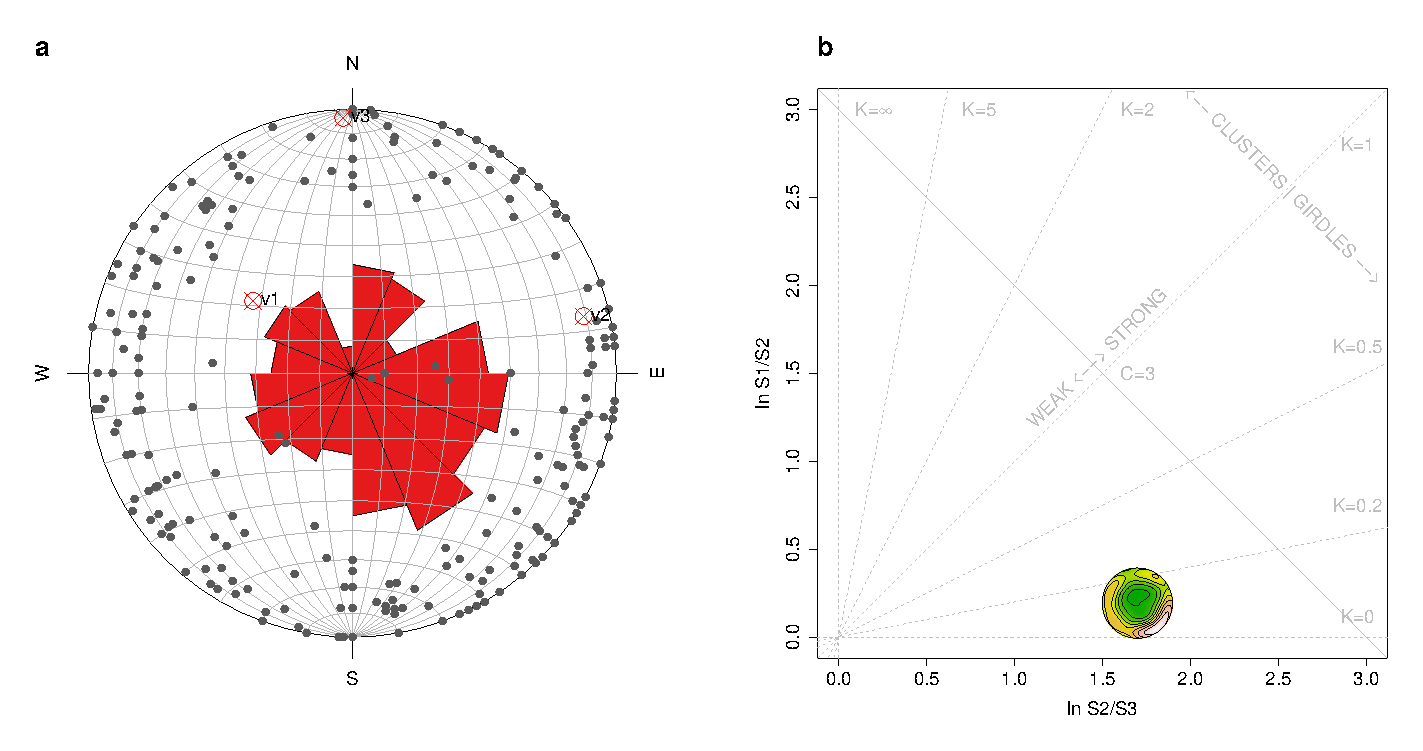
\includegraphics[width=1\textwidth]{./artwork/Fig5.pdf}
  \caption{Rose and equal area Schimdt diagrams (a). Woodcock diagram (b).}
  \label{fig:fabric}
\end{figure}

\subsection{Anisotropy of the taphonomic population}

%% Kernel density, Multidirectional variogram & Variogram map
Geostatistics (directional variograms and variogram map), wavelet and point pattern analyses were used for detecting anisotropy at the assemblage level. Fig.~\ref{fig:gstat}a shows the kernel smooth density estimation ($\sigma=0.17$) of the sample distribution in the study area. A preliminary visual examination suggests a NW-SE oriented clustering of the assemblage, although interfered with secondary NE-SW oriented dispersion. Fig.~\ref{fig:gstat}b shows the variograms in the four main geographical directions (N-S, E-W, NE-SW, NW-SE), plotted against the omnidirectional fitted variogram. As a rule of thumb, in order to determine the spatial structure of the sampled data, only the first two-thirds of the variogram are interpreted \citep{Dale2014}. The omnidirectional variogram (red line) indicates that at short distance lags, the semi-variances are close to zero, indicating very strong spatial structure (correlation). With longest distance lags, the semi-variance rise to a plateau (\emph{sill}) of lack of spatial correlation. The semi-variance of the NW-SE (135°) direction is lower than in the omnidirectional variogram, starting well before the \emph{sill}, thus indicating continuity (spatial correlation) in that direction. Minor directional trends are also detected in the N-S (0°), and to a lesser extent in the NE-SW (45°) directions. This result is clearly confirmed by the diagonal striping in the variogram map (Fig.~\ref{fig:gstat}c). The map shows a major ellipse oriented NW-SE, with minor parallel structures.

\begin{figure}
  \centering
  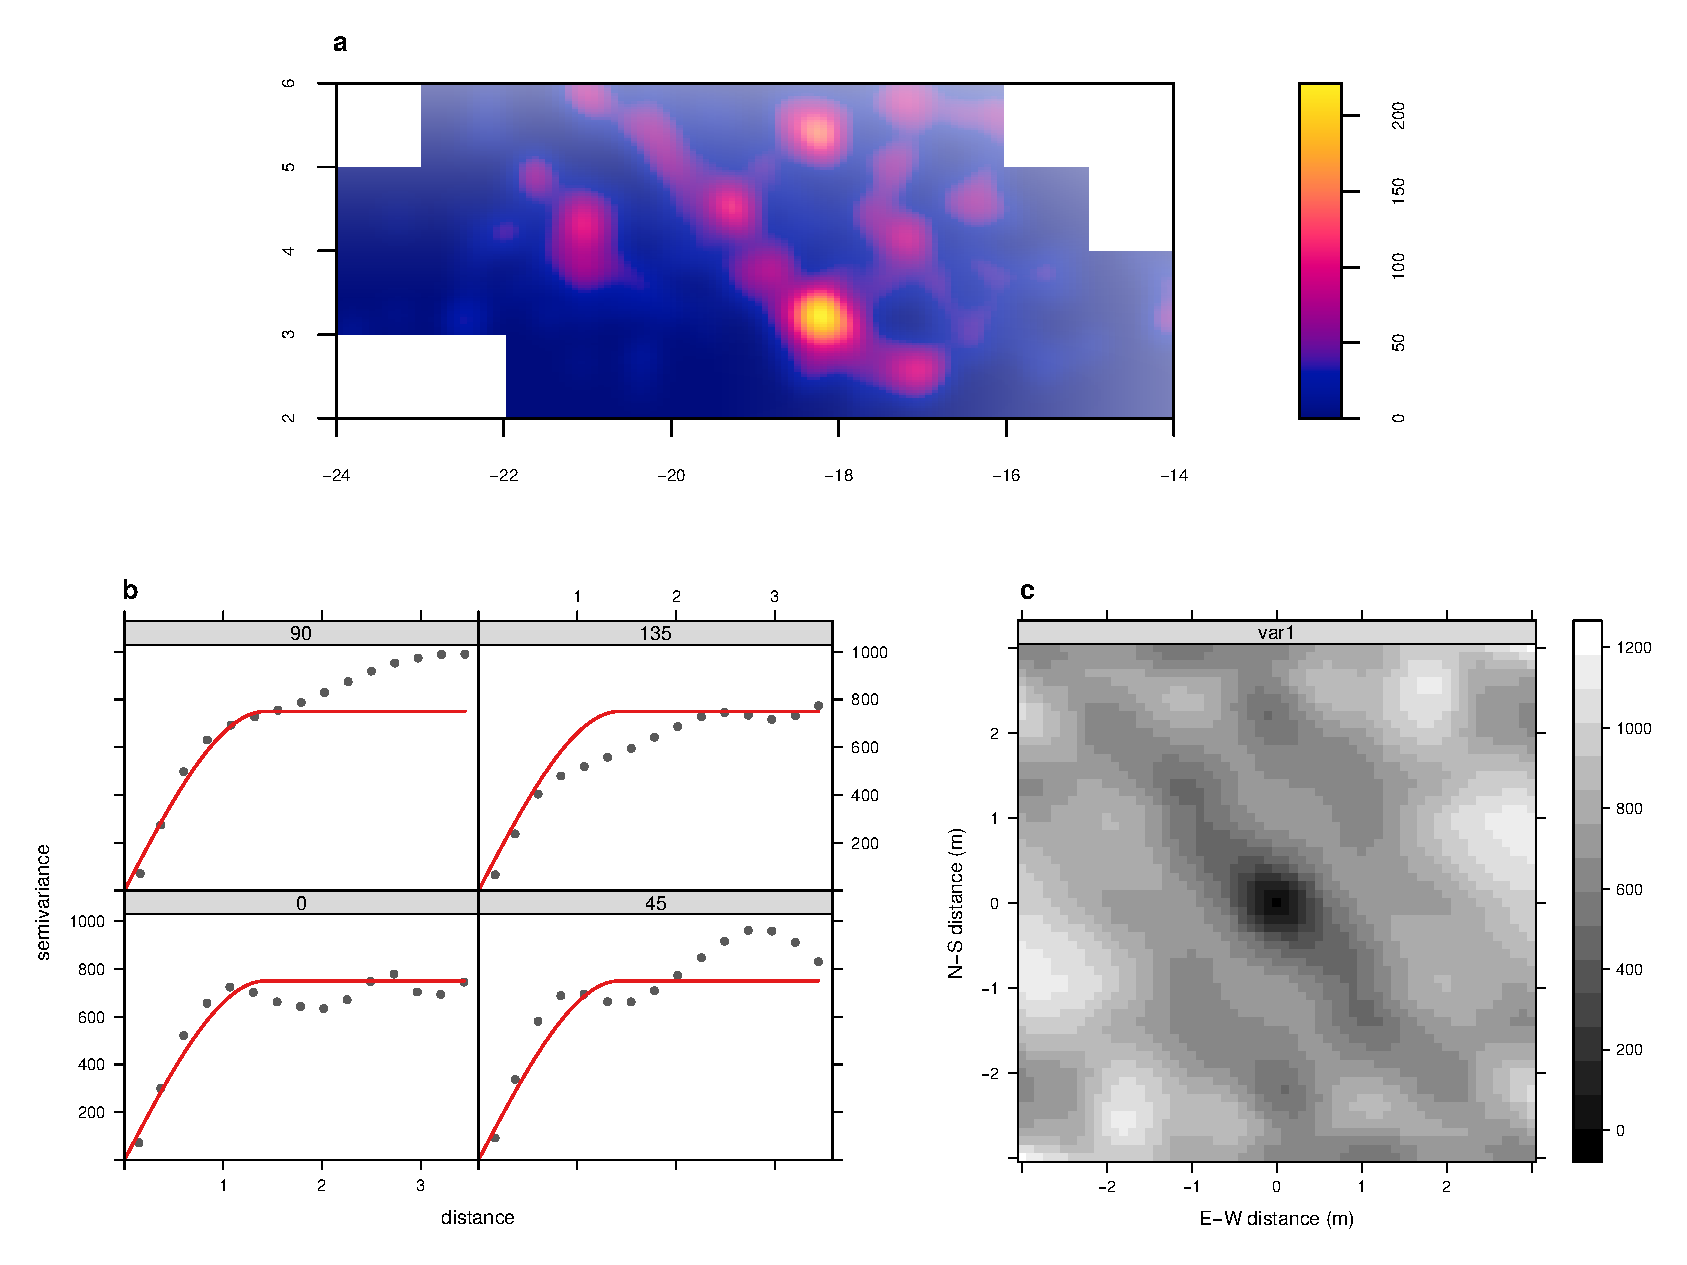
\includegraphics[width=1\textwidth]{artwork/Fig6.pdf}
  \caption{Kernel smoothed intensity function of the fossil assemblage (a). Directional variograms (4 clockwise directions from N-S, 0°) shown as grey points alongside the fitted omnidirectional variogram shown as a continuous red line (b) and variogram map (c).}
  \label{fig:gstat}
\end{figure}

%% Wavelet analysis
As for the wavelet analysis, Fig.~\ref{fig:wave} plots the variance as function of the direction, ranging anti-clockwise from 0° (E) to 180° (W). A major peak is evident at 135° (NW), wandering way above the expected values for a random (isotropic) pattern. A secondary significant peaks, although of much less intensity, is present at 85° (N). In accordance with the directional variograms, the wavelet analysis indicates a significant anisotropy in the NW-SE direction. Moreover, it suggests minor occurrence of points (specimens) in the N-S direction, as also indicated by the geostatistics analysis. However, in contrast with the directional variograms, the angular wavelet graph does not support significant preferential orientation in the NE range (angles between 0° and 90°).

\begin{figure}
  \centering
  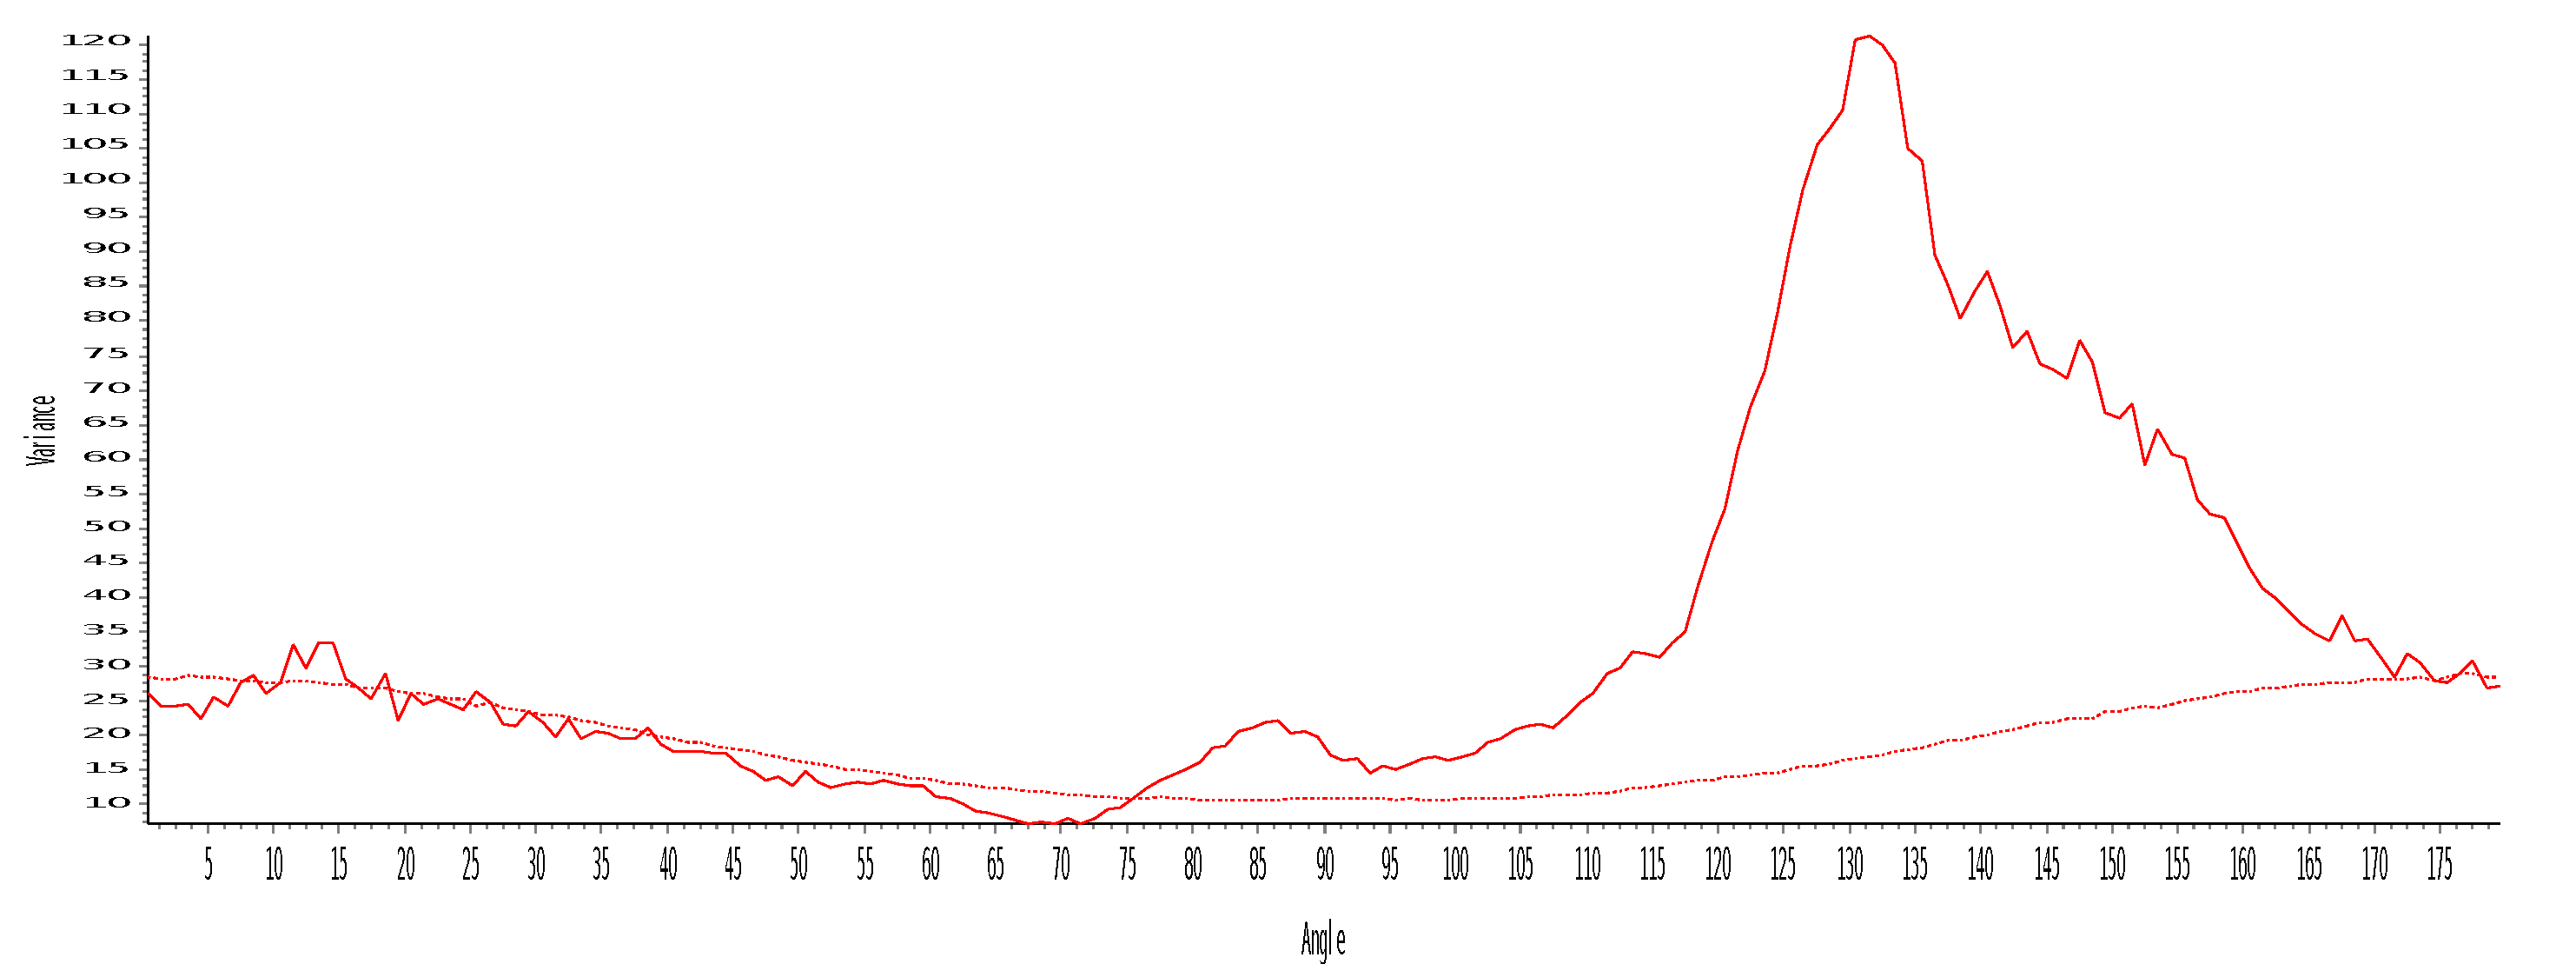
\includegraphics[width=1\textwidth]{artwork/Fig7.pdf}
  \caption{Angular wavelet graph. Angles range from 0° (E) to 180° (W). Peaks of variance (continuous line) indicate the direction of maximum anisotropy. Dashed line marks the Monte Carlo simulated null hypothesis of isotropy.}
  \label{fig:wave}
\end{figure}

%% Point pattern analysis
Fig.~\ref{fig:ppp} shows the results of our point pattern analysis and specifically the point pair distribution function $O_{r1,r2}(\Phi)$ for a range of distances $r1=0.01$ m and $0.25<r2<1.5$ m. The plot illustrates the multiscale variation of anisotropy, from a uniform, isotropic pattern (for $r2=0.25$ m), to increased anisotropy in the NW-SE direction. The maximum anisotropy is observed for $r2=1$ m, as elements at a maximum distance of 1 m show the strongest directional pattern. With increased distances of $r2>1$ m, the rose diagrams suggest the addition of a second orthogonal NE-SW directional trend, which reflects the parallel alternation of NW-SE bands in the assemblage distribution.

\begin{figure}
  \centering
  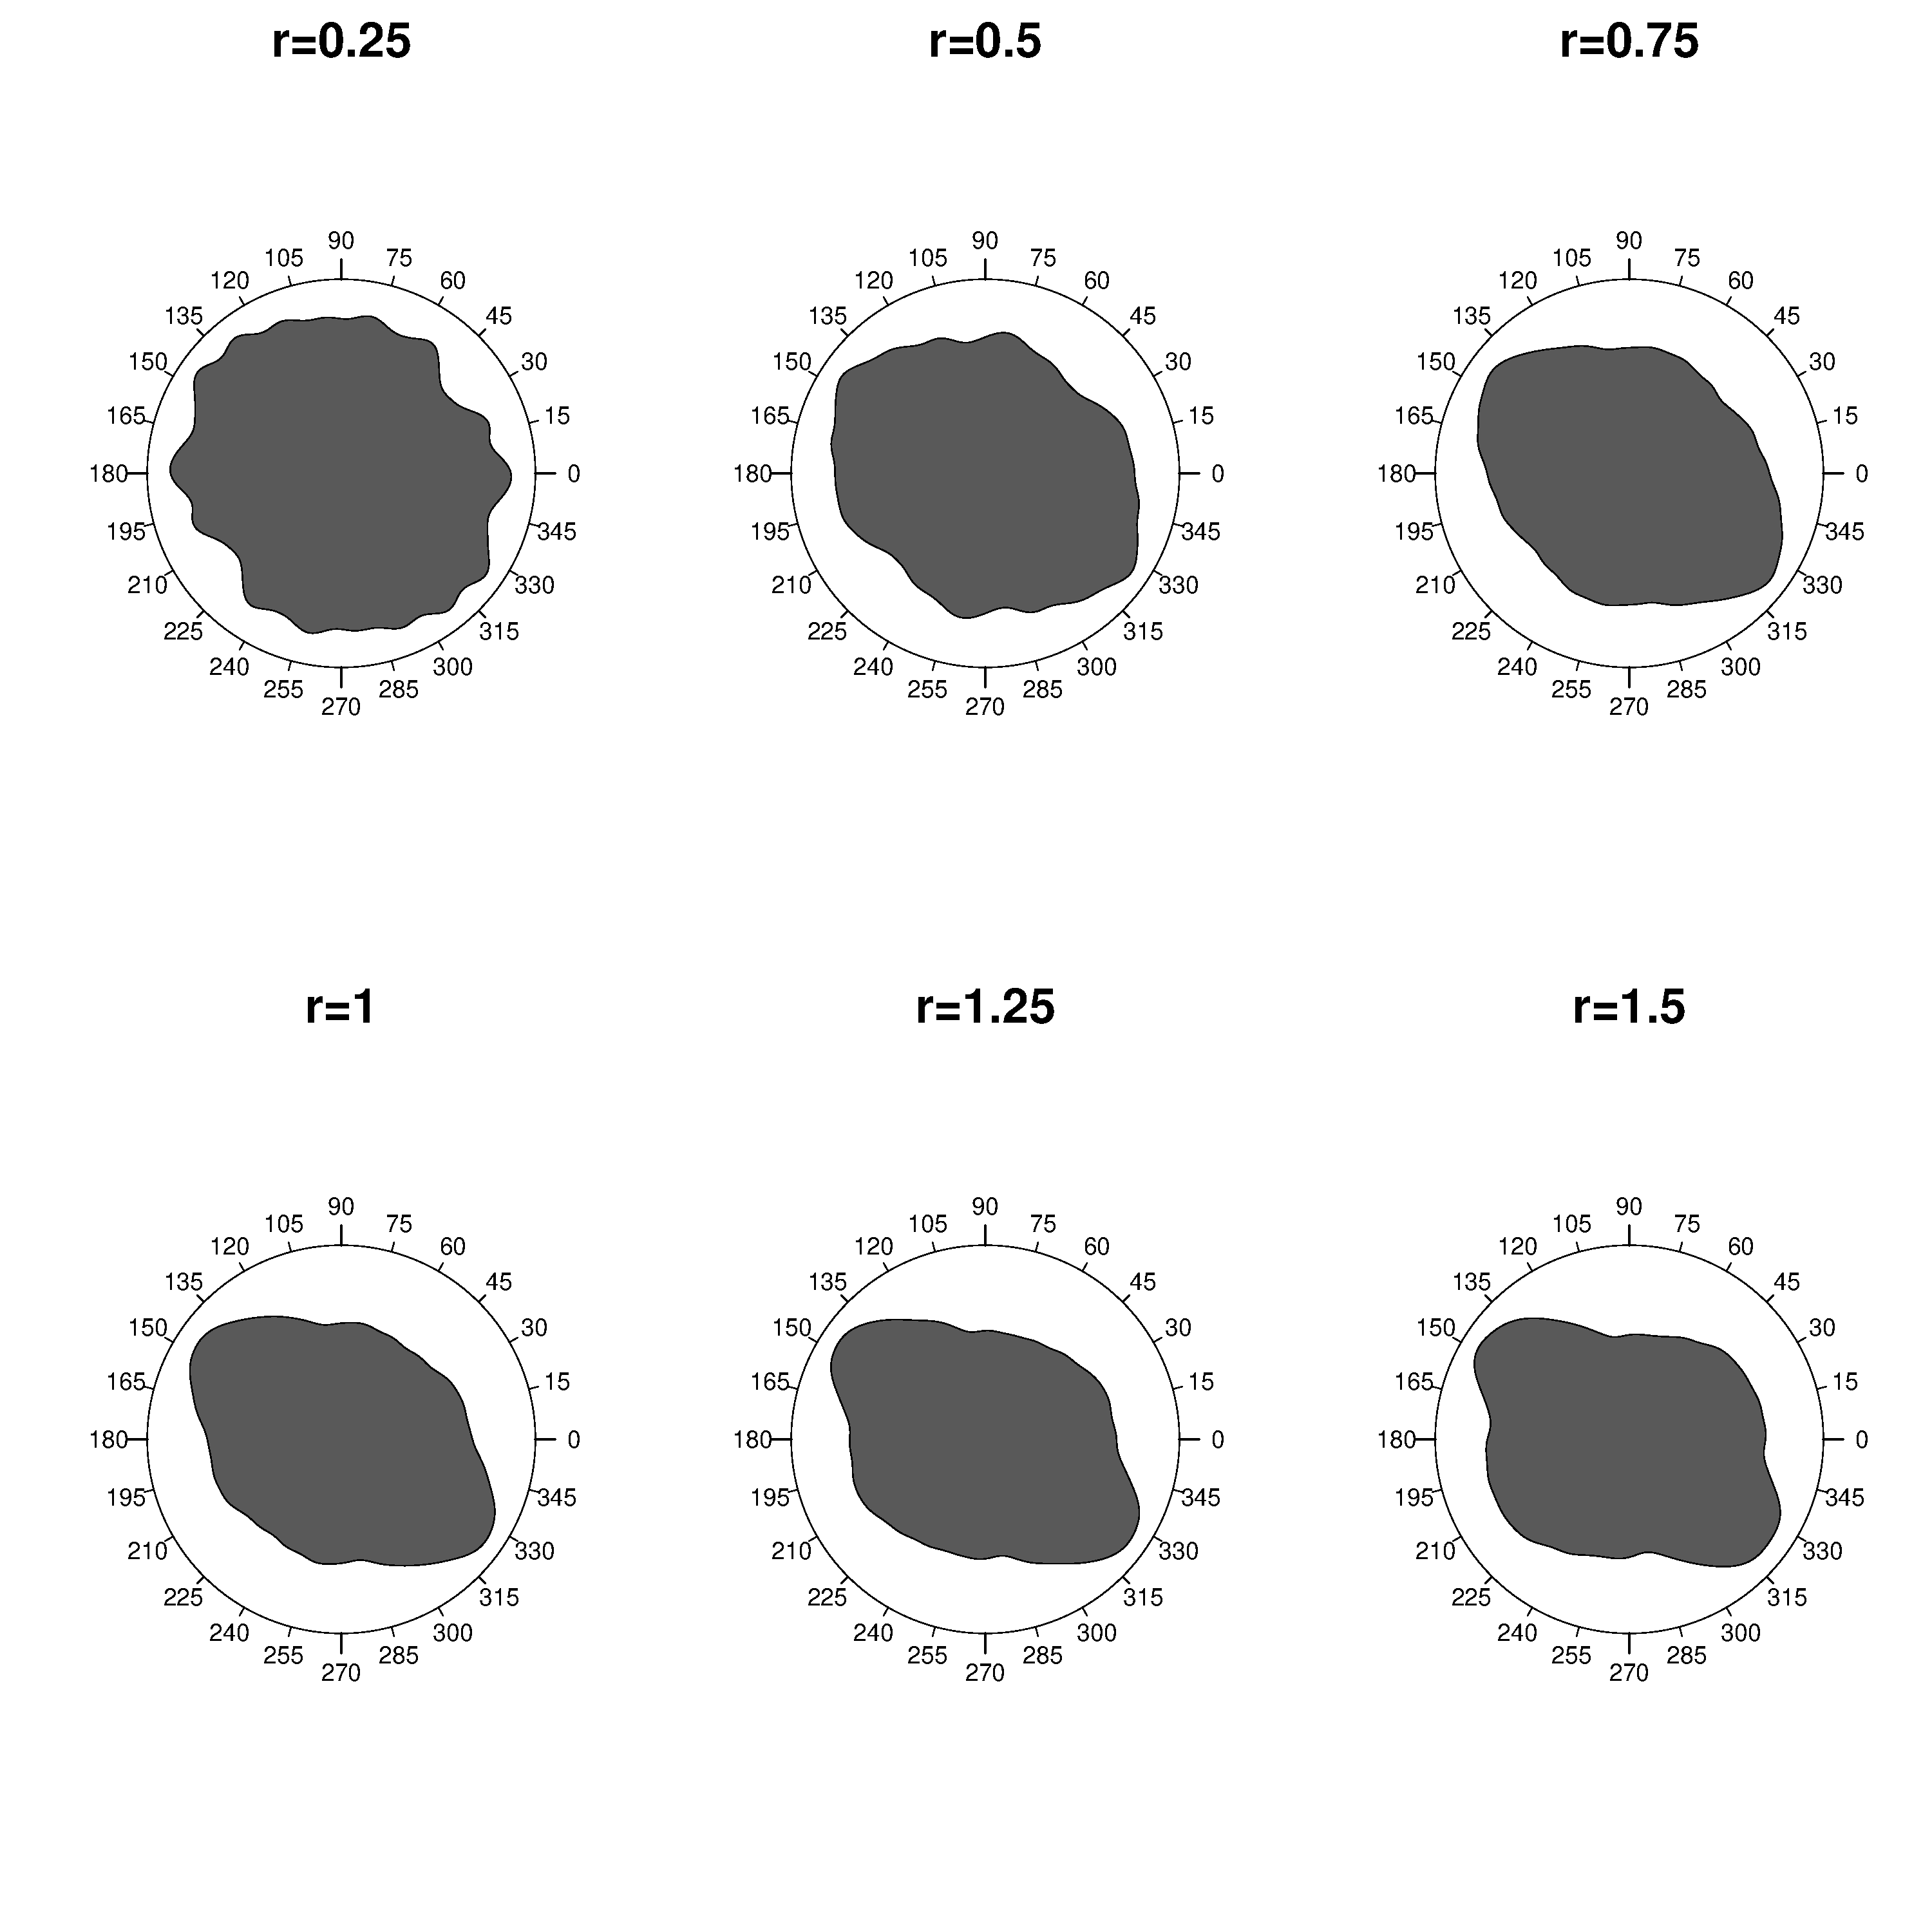
\includegraphics[width=1\textwidth]{artwork/Fig8.pdf}
  \caption{Rose diagrams of the point pair distribution function for a range of distances ($0.25<r2<1.5$m). Direction is measured counter-clockwise from East (0°).}
  \label{fig:ppp}
\end{figure}

\subsection{Anisotropy of magnetic susceptibility}

In Fig.~\ref{fig:ams}a, the AMS of the whole sample set (n = 18) is investigated. The equal-area projection of the three susceptibility axes K1-K3 (left-hand side of Fig.~\ref{fig:ams}a) indicates high variability of the axes orientation, with confidence angles of the K1 and K2 mean directions largely overlapping. This result suggests no preferential orientation of the axes. However, the Flinn and Jelinek plots (right-hand side of Fig.~\ref{fig:ams}a) reveal the presence of 7 samples with prolate ellipsoids, thus suggesting the action of post-depositional deformation processes which could have obliterated the primary depositional pattern. Therefore, in order to overcome possible post-depositional noise, further AMS analysis focused only on a sub-set of samples showing oblate ellipsoids (n = 11). In Fig.~\ref{fig:ams}b, the equal-area projection shows a well defined clustering of the axes, with the maximum anisotropy axis K1 aligned along the NW-SE direction and the K3 imbrication angles varying within a wide range of angles (from 4° to 85°). Because high K3 imbrication angles may result from post-depositional rehash of sediments, further analysis were conducted on a selection of 5 samples with K3 imbrication angles less than 20° \citep{Hamilton1970,Hrouda1982,Tarling1993,Liu2001,Lanza2006}. In Fig.~\ref{fig:ams}c, the equal-area projection indicates again a NW-SE orientation of the maximum anisotropy axis K1. Despite the small sample size, the AMS analysis suggests a weak anisotropy of magnetic sedimentary grains along a NW-SE direction.

\begin{figure}
  \centering
  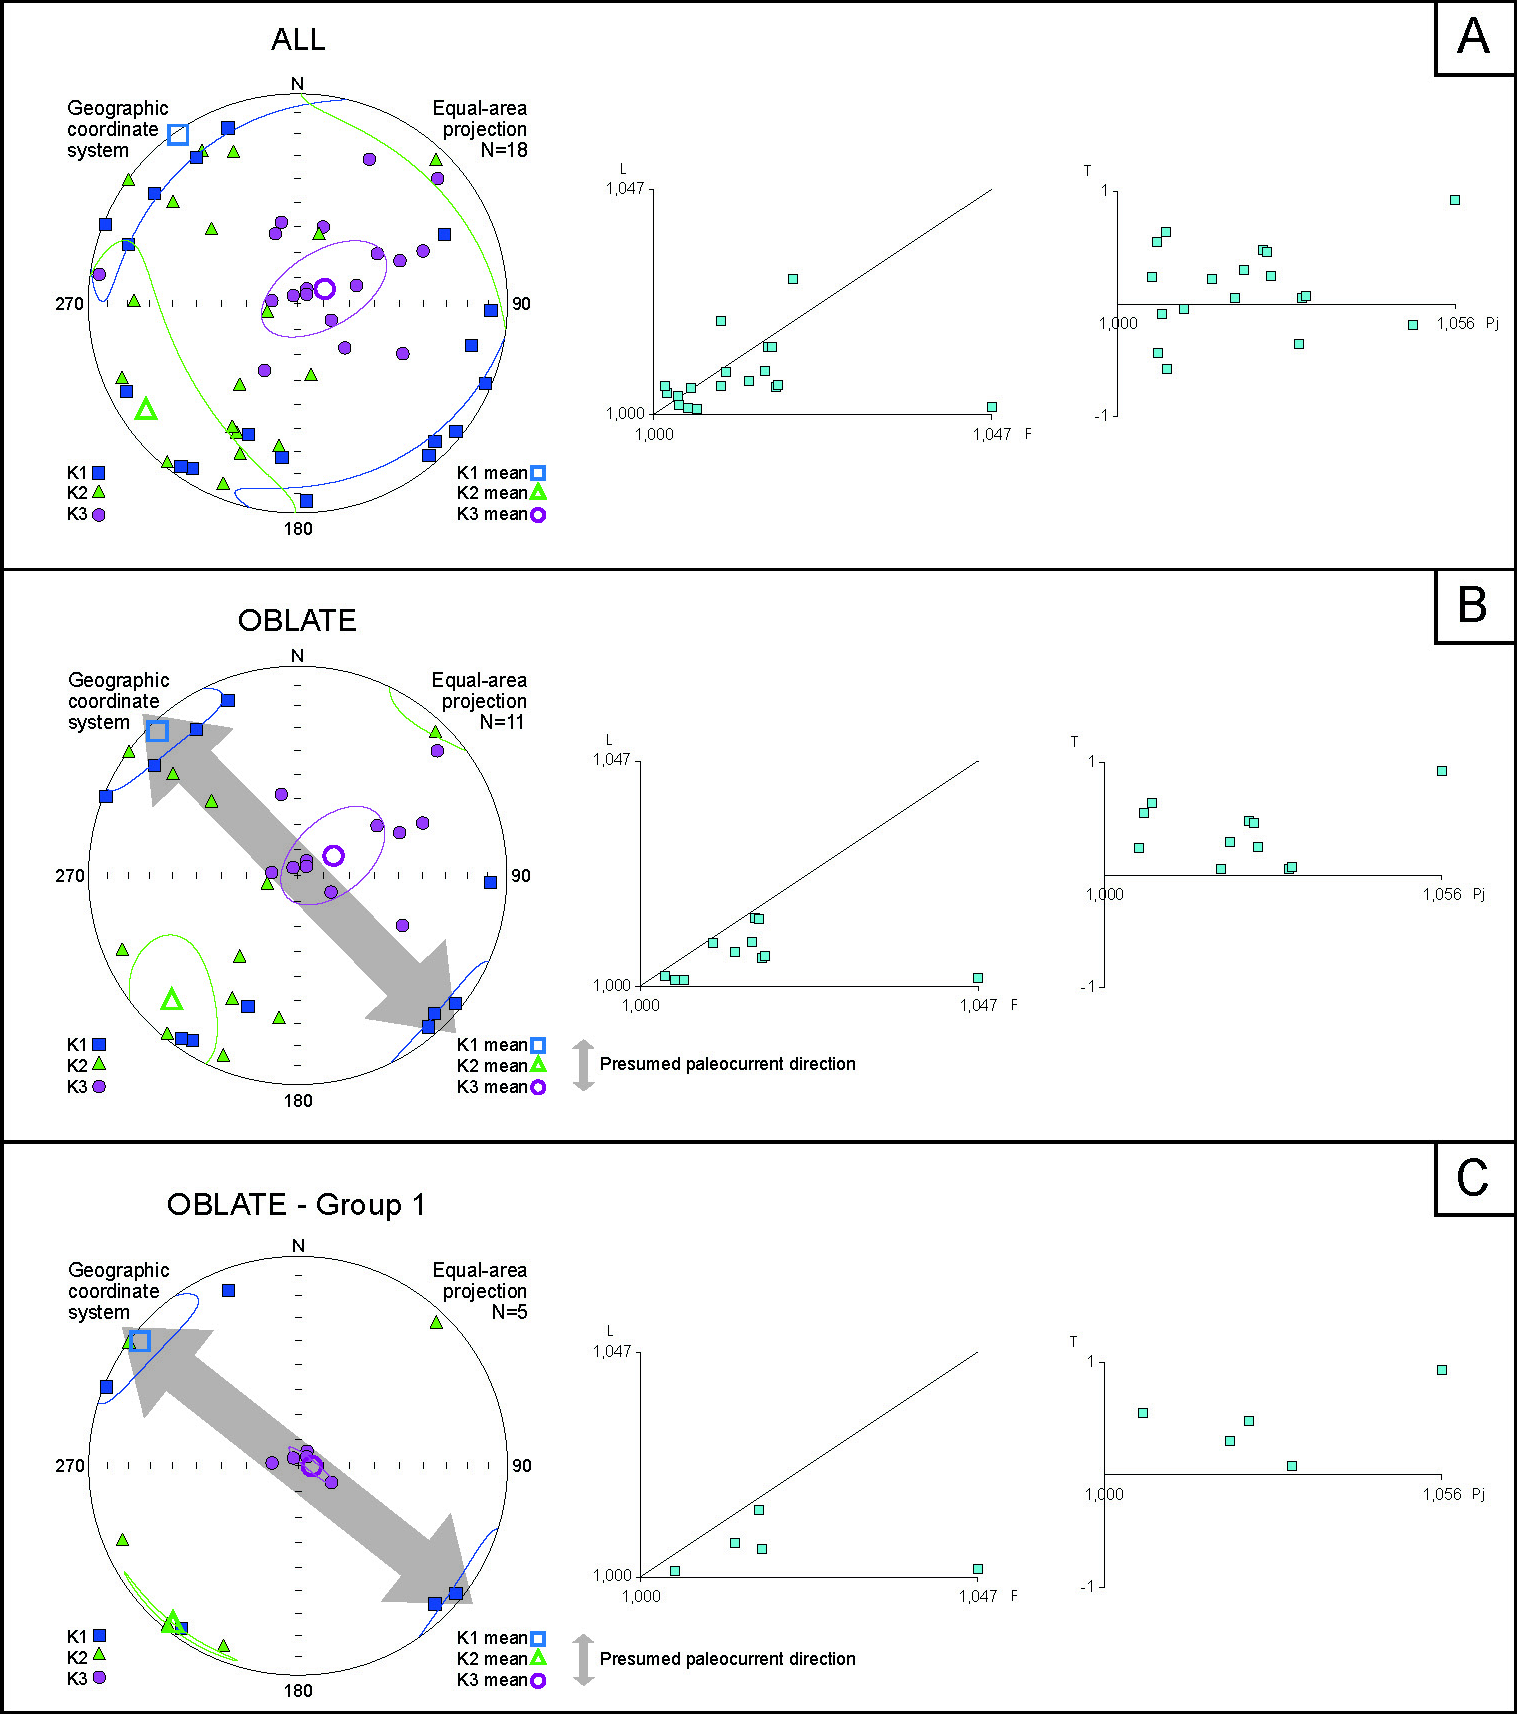
\includegraphics[width=1\textwidth]{artwork/Fig9.png}
  \caption{Equal-area projection stereogram (left-hand side) of the anisotropy axes K1, K2 and K3 (with K1 > K2 > K3) and Flinn and Jelinek plots (right-hand side) for a) all the samples; b) samples with oblate-shaped anisotropy ellipsoid; c) samples with K3 imbrication angle less than 20-25°.}
  \label{fig:ams}
\end{figure}

\subsection{Differential preservation}

%% Intro
Fig.~\ref{fig:fauna}a shows the distribution at the family level of the whole sampled material. Determined taxa included Perissodactyla, Artiodactyla, Carnivora and Proboscidea, together with a number of undetermined bone fragments (44\%). The histogram shows the prominent presence of Equidae over other taxa (27\%), followed by Bovidae (11\%) and Cervidae (5\%). However, it is worth noting the presence of very large mammals (body mass class BM5), such as Elephantidae and the rhinocerotid \emph{Stephanorhinus} sp., and to a less extent, of carnivores, such as \emph{Canis etruscus} and \emph{Ursus etruscus}.

%% Voorhies groups
The distribution of the Voorhies Groups plotted by body mass classes is shown in Fig.~\ref{fig:fauna}b. BM1 is so far not present in the TSR assemblage, while BM2 includes the \emph{C. etruscus}, BM3 includes the medium-sized Cervidae and \emph{Ursus etruscus}, BM4 the medium- and large-sized \emph{Equus} sp., \emph{Bison} sp. and the large-sized cervid \emph{Praemegaceros} sp. Notably, the Voorhies Group III is represented in Fig.~\ref{fig:fauna}b only by the crania of the carnivores \emph{Canis} and \emph{Ursus}. Moreover, the fossil record of \emph{U. etruscus} included maxilla fragments (Voorhies Group II/III), isolated teeth, 2 articulated vertebrae and an ulna fragment. Specimens from the BM4 grouped mostly in II/III, II, I/II and showed lack of Voorhies Group I and III. On the other hand, the bulk of undetermined BM specimens plotted in Voorhies Group I/II, with some occurrence in Group I, II, and to a less extent in Group II/III.

%% Skeletal element distribution
Fig.~\ref{fig:fauna}c shows the side-by-side distribution of complete and fragmented isolated macromammal skeletal elements. Firstly, the skeletal element distribution of complete specimens suggests a very high teeth/vertebra ratio (7.8). The ratio (3) is lower, but still relatively high when considering isolated, fragmented specimens. Limb bone and undetermined fragments represent the majority of the fragmented, isolated specimens, as compared to axial skeletal parts.

%% Articulated specimens
Accordingly, the prominent presence of appendicular skeletal elements over axial is also showed in the distribution of articulated specimens (Fig.~\ref{fig:fauna}d), which account for 22\% of the sampled assemblage. Articulated lower limb elements (metapodes, carpals/tarsals, phalanges) represent the majority of bones, often articulated to fragmented upper elements (radii, tibiae, humeri, femora). Interestingly, some of the latter elements present carnivore gnawing marks (Fig.~\ref{fig:pics}e).

\begin{figure}
  \centering
  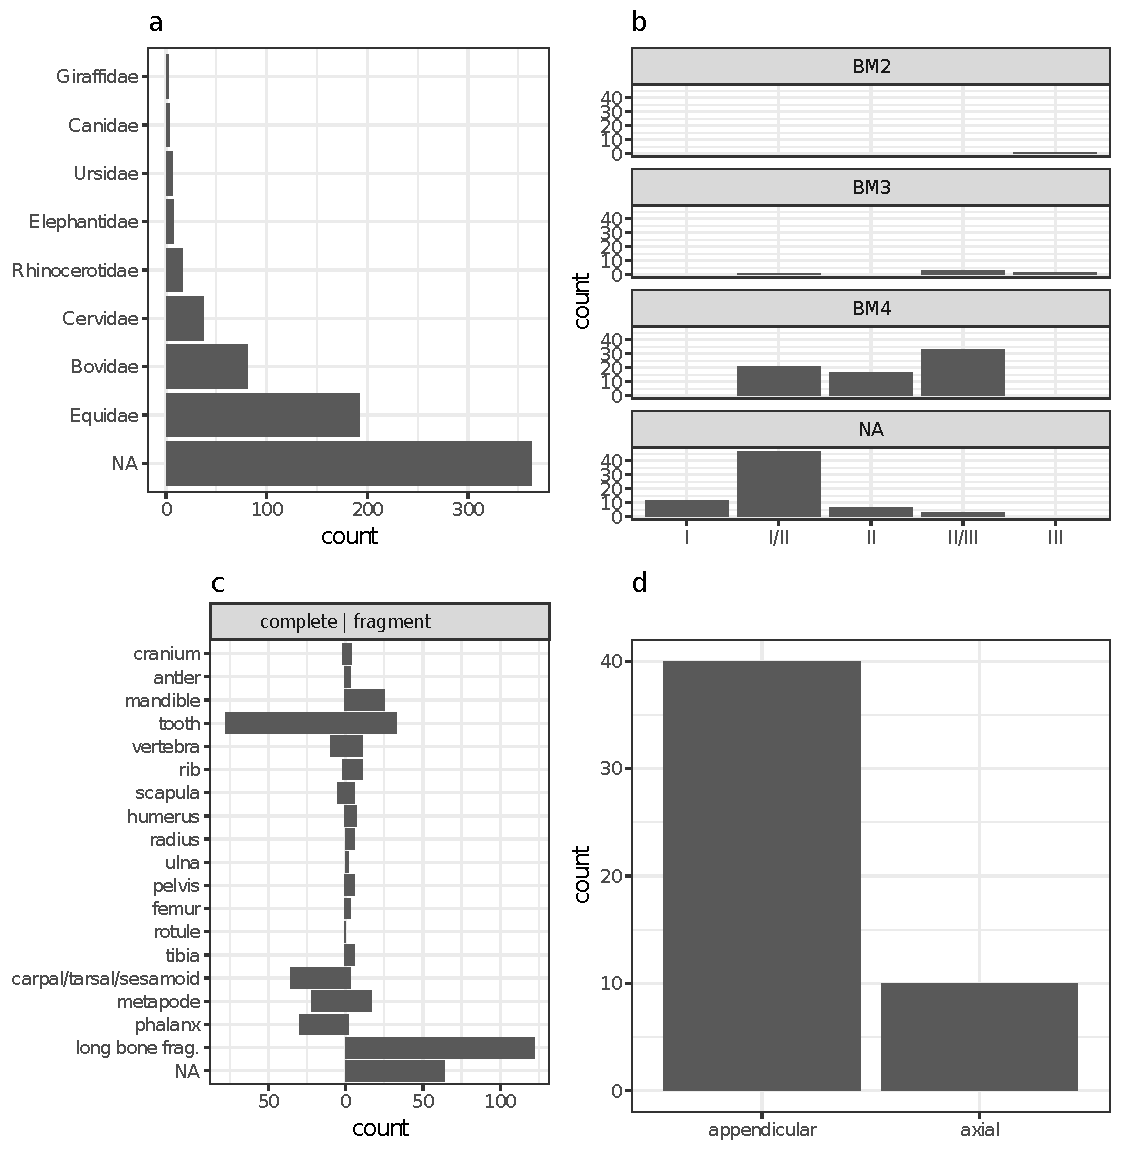
\includegraphics[width=1\textwidth]{artwork/Fig10.pdf}
  \caption{Distribution at the family level of the whole sampled material (a). Voorhies Groups distribution of the complete, isolated macromammal bones (plus rami of mandibles and maxillae) by body mass (BM) (b). Side-by-side distribution of complete/fragmented isolated macromammal skeletal elements (c). Skeletal region distribution of articulated macromammal specimens (d).}
  \label{fig:fauna}
\end{figure}

\subsection{Micromorphology}

The TVB-Z 1 block (Fig.~\ref{fig:log}) consists mostly of poorly sorted sandy silts, compositionally dominated by metamorphic quartz and accessory metamorphic minerals. From bottom to top, several sharp grain size breaks occur, which partition the sampled interval into mm-thick normally graded laminae, displaying an upward increase of matrix content (Fig.~\ref{fig:micro}a). This includes clay infilling pore spaces (Fig.~\ref{fig:micro}a) and suggests either flow velocity fluctuations or multiple waning depositional events. Birefringent illuvial clay coatings are also present along some voids (Fig.~\ref{fig:micro}b), thus indicating incipient pedogenesis, likely due to temporary subaereal exposure \citep{Kuehn2010}.

Most of the thickness of the TVB-Z 2 block (Fig.~\ref{fig:log}) displays similar characteristics to the TVB-Z 1 block, except for the presence of rolled soil clasts (pedorelicts; Fig.~\ref{fig:micro}c), likely eroded from nearby locations \citep{Cremaschi2018}. Conversely, the uppermost part of the sample (Fig.~\ref{fig:micro}d) displays moderate clay illuviation along voids, sparse voids most likely related to bioturbation and impregnating redoximorphic features \citep{Lindbo2010}. The latter include Fe oxide hypocoatings on the groundmass, Fe/Mn oxide nodules with regular outline developed on quartz grains, and fragmented clay coatings. Altogether, these features suggest that, after deposition, Geo 2a underwent moderate pedogenesis due to a relatively prolonged phase of subaereal exposure in a warm and possibly humid climate or while still saturated with water.

\begin{figure}
  \centering
  \includegraphics[width=1\textwidth]{artwork/Fig11.png}
  \caption{Microphotographs showing a) clast alignments (dashed white lines), crude normal grading and clays infilling pore spaces (arrows) from block TVB-Z 1 in parallel polarised light (PPL); b) illuvial clay coating a planar void from sample TVB-Z 1 in cross polarised light (XPL); c) rolled pedorelict (a Fe/Mn nodule developed on quartz grain) from topmost part of block TVB-Z 2 (PPL); d) Fe oxide hypocoatings on the groundmass and illuvial clay coating of voids from topmost part of block TVB-Z 2 (XPL).}
  \label{fig:micro}
\end{figure}

\section{Discussion}

%% Intro
Spatial taphonomy has recently emerged as a new methodological framework complement to the traditional taphonomic approach \citep{Dominguez-Rodrigo2017}. By using spatial statistical methods, spatial taphonomy aims to investigate the multiscale and multilevel spatial properties of different taphonomic entities \citep[\emph{sensu}][]{Fernandez-Lopez2006}. Indeed, taphonomic alteration processes work simultaneously, at different scales, on entities of different level of organisation, from the basic taphonomic elements (bone specimens), to higher level taphonomic groups (taphons) or populations (assemblages). For example, dispersion processes of taphonomic elements may modify their spatial location, orientation and removal degree. At the same time, dispersion of taphonomic elements may also cause changes in the density, spatial distribution and representatives of elements of each taphon or taphonic population \citep{Fernandez-Lopez2006}. Thus, beside the traditional taphonomic approach, the results of spatial taphonomy are of great importance for investigating the natural or cultural processes of dispersal and accumulation of faunal or cultural remains, in turn with consequences for palaeoecological reconstructions, biochronological estimates and past human behavioural inferences.

In this regard, this study offers an initial contribution to the development of a so far non-existent referential framework for the spatial taphonomic interpretation of palaeontological or archaeological assemblages \citep{Dominguez-Rodrigo2017}. Indeed, the taphonomic study of non-human related bone assemblages has great importance for archaeological research as well. As an example, water-flow processes are recognised to be among the most important natural processes in the formation and modification of a significant percentage of the vertebrate fossil and archaeological sites alike \citep[][among others]{Behrensmeyer1975,Behrensmeyer1982,Behrensmeyer1988,Coard1995,Coard1999,Petraglia1987,Petraglia1994,Schiffer1987,Voorhies1969}. Under the effect of water-flows, assemblages may adopt a variety of forms, ranging from (peri)autochthonous rearranged assemblages and biased lag assemblages to transported, allochthonous assemblages \citep{Behrensmeyer1988,Dominguez-Rodrigo2013}. One fundamental assumption behind reliable inferences on past human behaviour is the pristine preservation of the depositional context. Therefore, it is essential, in order to fully comprehend the archaeological record, to test within a referential framework alternative taphonomic hypotheses.

In this study, taphonomic dispersion and accumulation processes were analysed focusing on a specific aspect - anisotropy - of the spatial properties of taphonomic entities. A multilevel analysis of anisotropy was conducted at the level of basic taphonomic elements and at the assemblage level. Anisotropy, defined as the preferential orientation of skeletal elements, constitutes a fundamental part of any taphonomic study \citep[][among others]{Toots1965,Voorhies1969,Nash1987,Schick1987a,Petraglia1987,Petraglia1994,Fiorillo1991,Benito-Calvo2011,Torre2013a,Dominguez-Rodrigo2012,Dominguez-Rodrigo2014,Dominguez-Rodrigo2014c,Cobo-Sanchez2014,Aramendi2017,Organista2017}. However, spatial anisotropy at supra-element level of taphons or assemblages is an often neglected taphonomic criterion that should be reconsidered, especially in spatial taphonomic analyses of fluvial dispersion and accumulation processes. Nevertheless, standard spatial statistics rely on crucial assumptions about the isotropy of the spatial processes responsible for the observed spatial pattern \citep{spatstatBook}.

We investigated the multilevel spatial anisotropy and selective composition of the fossiliferous deposit of Tsiotra Vryssi, from the fluvial Gerakarou Formation of the Mygdonia Basin, Greece. Specific research questions regarded the character and number of depositional processes and the degree of re-elaboration of the fossil record. Specific aspects of our results are discussed below.

\subsection{Recursive anisotropy}

%% Intro
Recursive anisotropy emerged at the level of basic taphonomic elements and at the assemblage level. Fabric analysis, geostatistics, wavelet and point pattern analyses all pointed to a preferential NW-SE orientation of the assemblage and the sub-sample of elongated bone specimens.

%% Anisotropy of basic taphonomic elements
Fabric analysis, or the analysis of the orientation (plunge and bearing) of elongated elements, can provide valuable insight into taphonomic processes, allowing discrimination between different orientation patterns (isotropic, linear or planar). We analysed a sub-sample of not articulated, clearly elongated bone specimens, mostly limb bone fragments. Articulated units were excluded from the fabric analysis since experimental studies by \cite{Coard1995} and \cite{Coard1999} reported that articulated units with a higher number of elements, such as complete limbs, may show weak preferential orientation when not aligned, as they often occur at TSR (Fig.~\ref{fig:pics}c,d,e). Otherwise, the authors concluded that articulated bones showed a greater than expected hydraulic transport potential. Thus, their conspicuous presence in the TSR fossil record (about 22\%) would not necessarily suggest an autochthonous deposit.

The results of the circular uniformity test statistics (Tab.~\ref{tab:1}) agreed upon rejecting the null hypothesis of uniformity, suggesting a significant anisotropic distribution of the fossil sample. The Schimdt and Woodcock diagrams in Fig.~\ref{fig:fabric} indicated planar fabric (0-to-low degree of dip) and a girdle pattern, with preferential orientation towards the SE. In girdle distribution elements orient over a wider sector of angles than cluster distributions, yet showing higher anisotropy than random distributions. Whereas cluster, linear patterns are associated with channelised water-flows \citep{Petraglia1994}, girdle, planar patterns have been interpreted as products of overland flows (runoff; \citealp{Organista2017}). The preferential orientation of the sampled elongated bones suggests that the TSR fossil deposit most likely underwent relatively high-energy, but non-channelised NW-SE water-flows. However, anisotropy does not itself discriminate between allochthonous and autochthonous deposits. Autochthonous lag assemblages undergoing minimal re-sedimentation could also exhibit significant anisotropic spatial patterns \citep{Dominguez-Rodrigo2012,Dominguez-Rodrigo2014a,Dominguez-Rodrigo2014b,Dominguez-Rodrigo2017}. Since a wide range of different taphonomic processes can produce similar patterns, an unequivocal discrimination based only on fabric observations is seldom possible, and other taphonomic criteria should be considered \citep{Lenoble2004}.

%% Anisotropy of the taphonomic population
Geostatistics, wavelet and point pattern analyses were applied in order to detect anisotropy of the TSR fossil assemblage. All these different methods agreed on identifying a preferentially NW-SE oriented distribution. Four directional variograms and a variogram map (Fig.~\ref{fig:gstat}b,c) were calculated from a kernel density estimation of the assemblage spatial distribution (Fig.~\ref{fig:gstat}a). Small, dense clusters of fossils, although occurring at different elevations in the 1m-thick vertical distribution (Fig.~\ref{fig:map}a), concatenate along a prevailing NW-SE direction. Secondary minor directions (N-S and NE-SW) were identified in the directional variograms (Fig.~\ref{fig:gstat}b). In the same manner, the wavelet graph (Fig.~\ref{fig:wave}) and the rose diagrams (Fig.~\ref{fig:ppp}) also detected a strong preferential NW-SE directional distribution. Similar elongated lag deposits are typically associated with water-flows dragging material in one direction \citep{Dominguez-Rodrigo2012}.

These observations are in agreement with the AMS results. Despite the small sample size, the AMS results suggest relatively strong anisotropy, with a mean K1 axis oriented NW-SE and a mean K2 axis oriented NE-SW, although with much smaller confidence angles (Fig.~\ref{fig:ams}). Since K1 (i.e., the axis of maximum anisotropy) should reflect the bulk orientation of the elongated axis of the ferro/paramagnetic sedimentary particles, it might be concluded that AMS hints at a NW-SE oriented anisotropy.

%% Recursive anisotropy and clustering patterns
Thus, the observed recursive multilevel anisotropy patterns most probably points to the action of NW-SE oriented water-flows, at the specific location of the TSR site. However, both analyses of isotropy at element level (fabric analysis) and assemblage level (geostatistics, wavelet and point pattern analyses) suggested some degree of noise in the prevalent NW-SE distributions toward other directions, especially to the orthogonal NE-SW direction. Whereas long bones can roll orthogonally to the main direction of the flow \citep{Voorhies1969}, noise in the main directional trend at assemblage level may indicate multiple depositional processes, or secondary reworking post-depositional processes. Moreover, the relatively high average density of preserved elements (24/m$^2$) occur in small, well defined clusters (Figs.~\ref{fig:pics}f,e, \ref{fig:map} and \ref{fig:gstat}a). Such spatial aggregation of taphonomic elements may be the result of a combination or the sum of different taphonomic processes \citep{Fernandez-Lopez2002}. On the other hand, the formation of gaps in the spatial distribution and clusters of elements in correspondence with topographic depression may as well be associated with lag deposits \citep{Petraglia1994}. This is likely to happen on top of rippled surfaces or small dunes in the channel-belt. However, there is no evidence of such structure at TSR.

\subsection{Differential preservation}

%% Intro
According to the evolutionary and systemic theory of taphonomy, taphonomic alteration is not only conceived as a destructive process, but it also has positive effects with the preservation and creation of new taphonomic groups. In this sense, the differential destruction (or taphonomic sieve) of taphonomic entities is just a particular case of taphonomic alteration, as it is the differential modification that gives rise to selective preservation \citep{Fernandez-Lopez2006}. Intrinsic and extrinsic taphonomic factors determine the differential preservation of taphonomic entities. In this study we integrated our spatial taphonomic approach with a preliminary study of the differential preservation of fossil elements.

%% Voorhies Groups & T/V
In the BM4 class of mammals, the relatively high abundance of skeletal elements belonging to the Voorhies Groups I/II, II and II/III (Fig.~\ref{fig:fauna}b) suggests minor winnowing of the assemblage, with preservation of the densest elements that are above the threshold of transportability \citep{Behrensmeyer1988}. Indeed, skeletal elements in the Voorhies Group I (ribs, vertebrae, sacrum, sternum) tend to be transported more easily by saltation or flotation in relatively low-energy currents \citep{Voorhies1969}. The under-representation of the Voorhies Group III (crania and complete mandibles) in the BM4 class is balanced by the high occurrence of cranial elements in the Group II/III (rami of mandibles and maxilla fragments). Thus, the distribution in Fig.~\ref{fig:fauna}b suggests, more than the taphonomic sieve of the Voorhies Group III, a higher fragmentation rate of cranial elements in the BM4 class of mammals (\emph{Equus}, \emph{Bison}, \emph{Praemegaceros}). On the other hand, the Voorhies Group III is better represented in the BM classes 2 and 3, which include smaller mammals, i.e., \emph{C. etruscus}, \emph{U. etruscus} and medium-sized cervids. The presence of better preserved carnivore cranial elements, as well as the presence of a partial articulated skeleton of a wolf-sized carnivore, would suggest an autochthonous or para-autochthonous assemblage \citep{Behrensmeyer1988}.

Although excluded from the Voorhies Group analysis, it is worth noting the presence of several mostly complete skeletal elements of Elephantidae (e.g., ribs, scapula, humerus and several articulated carpals, metacarpals and phalanges) with different FTI values, comparable to elements of the Voorhies Group II and III \citep{Frison1986}. Their distribution suggests that the assemblage was winnowed of the elements with highest FTI, which are comparable to elements of the Voorhies Group I. This is also the case for the other excluded megaherbivore, the rhinocerotid \emph{Stephanorhinus}, which is represented by several teeth and limb bones.

%% Fragmented skeletal elements (size distribution)
Overall, the very high teeth/vertebra ratio (7.8) also supports the hypothesis of a lag, winnowed assemblage. Moreover, the actual presence of a high number of limb and undetermined bone fragments, together with complete appendicular and axial elements (Fig.~\ref{fig:fauna}c) supports also some degree of sorting (taphonomic sieve) of the smallest, cancellous fragments. Segregation of axial elements from epiphyses and shafts has been observed even in low-energy fluvial environments \citep{Dominguez-Rodrigo2017}.

%% Articulated units
On the other hand, as noted earlier, the conspicuous presence of articulated specimens in the TSR fossil assemblage does not necessarily suggest an autochthonous deposition, since articulated bones may as well show a great hydraulic transport potential \citep{Coard1995,Coard1999}. Nevertheless, it is worth noting that the distribution of articulated units at TSR shows a significant presence of appendicular elements over axial ones (Fig.~\ref{fig:fauna}d). Thus, the under-representation of articulated axial elements also indicates a winnowed, lag assemblage formed by the densest and most resilient elements, with sieve and transport of part of the lighter and more cancellous elements. However, carnivore ravaging alike tends to eliminate or at least lead to under-representation of those skeletal elements (the less dense, axial elements) in the transport group most prone to be transported by water \citep{Voorhies1969,Dominguez-Rodrigo2012}. Interestingly, a preliminary analysis of the bone breakage patterns suggests that carnivores had some active role in the modification and possibly in the accumulation of bones at TSR (Fig.~\ref{fig:pics}e; \citealp{Konidaris2015}).

%% Interpretation
In conclusion, considering the results of our spatial taphonomic analysis, processes of taphonomic dispersion, such as fluvial accumulation processes, would have likely separated and disseminated the most cancellous taphonomic elements, favouring the persistence of taphons constituted by allochthonous elements \citep{Fernandez-Lopez2006}. Carnivores could have likely been primary accumulation agents. However, the recursive anisotropic spatial patterns, at the level of taphonomic elements and at the assemblage level, as well as the clustering pattern in relatively small, dense, aggregations of elements aligned in parallel NW-SE oriented bands, suggest that the TSR deposit resulted from multiple taphonomic dispersion events, with winnowing of less dense, lighter elements and spatial anisotropic re-arrangement of a lag, autochthonous assemblage accumulated over the migrating banks of a NW-SE oriented fluvial system. As suggested by \cite{Organista2017}, it is likely for secondary over-bank flows to aggregate bones dispersed over the bank surface into topographic depressions, where they accumulate and acquire greater stability.

%% Mattia:
Noteworthy, both Geo 1 and Geo 2 show fining upward trends and facies sequences similar to those typical of braided rivers \citep{Miall1977}. In such a sequence, the lower coarser-grained part would represent one or more sets of sinuous-crested medium-scale bedforms (i.e., small dunes) forming by bedload traction in the deeper reaches of channels, whereas the upper muddy part is dominantly deposited by decantation either on top of in-channel or bank-attached emerging bars or in floodplains, occasionally provided with coarse material at high-water stages \citep{Miall1982}. Therefore, the excavated section can be viewed as the product of cyclical lateral switching of a braided fluvial system.

\section{Conclusions}

Spatial taphonomy is the systemic, multiscale and multilevel study of the spatial properties of taphonomic processes. Indeed, taphonomic alteration processes work simultaneously, at different scales, on entities of different levels of organisation, from the basic taphonomic elements (bone specimens), to higher level taphonomic groups (taphons) or populations (assemblages). In this study we elaborated on a specific aspect - anisotropy - of the spatial properties of taphonomic processes, investigating an often neglected aspect of the spatial distribution of taphonomic populations.

A multilevel analysis of anisotropy was conducted for the Early Pleistocene fossiliferous locality Tsiotra Vryssi, from the fluvial Gerakarou Formation of the Mygdonia Basin, Greece. Differential preservation of skeletal elements was also analysed in order to unravel the character and number of depositional processes and the degree of re-elaboration of the TSR fossil record. The results of the analyses suggested repeated taphonomic dispersion processes, with winnowing of less dense, lighter elements and spatial anisotropic re-arrangement of a lag, autochthonous assemblage possibly accumulated over the migrating banks of a NW-SE oriented fluvial system.

We believe that this study contributes towards the development of a referential framework for the spatial taphonomic interpretation of other palaeontological, as well as archaeological, localities.

\section*{Acknowledgements}

This research was supported by the European Research Council [ERC StG PaGE 'Paleoanthropology at the Gates of Europe: Human evolution in the southern Balkans' 283503, 2014] and [ERC CoG CROSSROADS 'Human Evolution at the Crossroads' 724703, 2017] awarded to K. Harvati. We are grateful to all the participants in the survey and excavation campaigns that took place in the Mygdonia Basin for their indispensable contribution. %We also thank ... and ... anonymous reviewers for their critical discussions and many constructive comments that helped to improve this manuscript.
 
\section*{References}

\bibliographystyle{elsarticle-harv}
\bibliography{tsr_rr}

\end{document}
